\documentclass[11pt,a4paper]{article}

\usepackage[margin=2.6cm]{geometry}
\usepackage{amsmath,amssymb}
\usepackage{graphicx}
\usepackage{booktabs}
\usepackage{xcolor}
\usepackage{mathpazo}
\usepackage[T1]{fontenc}
%\usepackage{microtype}
\usepackage{enumitem}
\usepackage[colorlinks=true, linkcolor=linkblue, urlcolor=linkblue, citecolor=linkblue]{hyperref}
\usepackage{caption}
\captionsetup{font=small, labelfont=bf, width=0.92\textwidth}

\definecolor{linkblue}{HTML}{1C5CAB}
\definecolor{accent}{HTML}{2A78D6}
\definecolor{inkgray}{HTML}{52514E}
\definecolor{boxbg}{HTML}{F4F6FA}

\newcommand{\E}{\mathbb{E}}
\newcommand{\Prob}{\mathbb{P}}
\newcommand{\Var}{\mathrm{Var}}
\newcommand{\dd}{\,\mathrm{d}}

\usepackage{mdframed}
\newmdenv[backgroundcolor=boxbg, linecolor=accent, linewidth=1.5pt,
  topline=false, bottomline=false, rightline=false,
  innertopmargin=8pt, innerbottommargin=8pt]{keybox}

\title{\vspace{-1.2cm}\textbf{Model Risk Lab}\\[4pt]
\Large What a Wrong Pricing Model Costs an Options Desk --- in Dollars\\[6pt]
\normalsize A market-making simulator calibrated to real SPY and NIFTY~50 data,\\
with a complete statistical model-validation suite}
\author{Arijit Ray \\ \small MSc Statistics, IIT Bombay \\
\small \texttt{github.com/Arijitray2/model-risk-lab}}
\date{\today}

\begin{document}
\maketitle

\begin{abstract}
\noindent
A market maker earns the bid--ask spread by quoting around \emph{fair value} --- but
fair value comes from a model, and the model can be wrong. This project measures that
danger end to end. Geometric Brownian motion (GBM) and the Merton jump-diffusion are
calibrated to 17+ years of SPY and NIFTY~50 daily returns by maximum likelihood
(GBM is rejected with likelihood-ratio statistics of $\approx1627$ and $\approx1313$)
and to four real SPY option chains --- on 16 March 2020 the options market priced
$\lambda=3.7$ crashes per year with mean size $-31\%$. A simulated options desk then
quotes a rolling three-month contract under four (true model, believed model)
scenarios with price-elastic client flow. When the model matches reality the desk
realises its quoted half-spread ($+0.153$ per contract against a promised $0.15$;
bootstrap 95\% CI $[0.146,0.159]$). When it prices Black--Scholes in the jump world,
it \emph{believes} it earns $+0.15$ while actually losing $10.20$ per contract, and
no half-spread below \$15 (${>}170\times$ the matched desk's break-even of
8.8~cents) makes it 95\%-safe. Finally, a validation suite --- Kupiec and
Christoffersen VaR backtests, bootstrap edge inference, and a CUSUM monitor ---
detects the broken model from realised P/L alone, raising an alarm at trade 83 of
1{,}467 with zero false alarms on the correctly-specified desk. All data, code,
figures and an interactive browser demo are in the repository. The write-up assumes
bachelor's-level probability and statistics; every model is stated with its
equations, and every design choice is explained by what it does to the final number.
\end{abstract}

\tableofcontents

%=====================================================================
\section{Introduction: the business of quoting, and its hidden bet}

\subsection{What a market maker does}
An options market maker continuously posts two prices for the same contract: a
\textbf{bid} at which it will buy and an \textbf{ask} at which it will sell. If the
option's fair value is $V$ and the desk quotes
\begin{equation}
\text{bid} = V - s, \qquad \text{ask} = V + s,
\end{equation}
then every client trade hands the desk $+s$ of expected profit (the
\emph{half-spread}): it sells above fair value and buys below it. Volume times $s$ is
the revenue of the business. This is real: option markets are quote-driven, and
market-making firms exist on exactly this economics.

\subsection{The hidden bet}
The catch is the symbol $V$. Nobody hands the desk fair value; it must be
\emph{computed from a model} of how the underlying asset moves. The desk's entire
P/L statement therefore rests on a modelling assumption that could be wrong. The
purpose of this project is to make the consequences of that assumption
\textbf{visible, measurable, and statistically testable}:
\begin{enumerate}[itemsep=1pt]
  \item \textbf{Calibrate} two competing models --- Black--Scholes/GBM and Merton
    jump-diffusion --- to real market data, with standard errors and formal model
    comparison (Section~\ref{sec:physical}--\ref{sec:rn}).
  \item \textbf{Simulate} a market-making desk that believes one model while the
    world follows another (Section~\ref{sec:desk}).
  \item \textbf{Measure} the damage in the units risk managers use: VaR, Expected
    Shortfall, drawdowns, and a break-even spread --- a dollar
    \emph{model-risk premium} (Section~\ref{sec:risk}).
  \item \textbf{Validate}: treat the desk's model as a hypothesis and reject it
    from realised P/L alone, using the same tests a bank's model-risk management
    (MRM) team runs --- Kupiec, Christoffersen, bootstrap, CUSUM
    (Section~\ref{sec:validation}).
\end{enumerate}

\begin{keybox}
\textbf{The one-sentence result.} A desk that prices Black--Scholes in a world with
COVID-sized jumps books $+0.15$ of ``edge'' per contract in its own accounting while
truly earning $-10.20$; statistical monitoring catches the lie within weeks, and no
commercially meaningful spread makes the wrong model safe.
\end{keybox}

\subsection{Origin and what is new here}
The seed of this project is a teaching simulator by Roman Paolucci (Quant Guild),
which demonstrates spread capture vs.\ model risk with assumed parameters and
price-blind client flow. This project rebuilds the idea as a statistics project:
all parameters are \emph{estimated} from real data with quantified uncertainty;
client flow is \emph{price-elastic} (mispricing attracts informed flow instead of
being ignored); the desk quotes a \emph{rolling constant-moneyness} contract so its
economics are stationary; and the headline contribution is the \emph{validation
layer} --- the machinery for detecting a wrong model from outcomes, which is the
day job of model validation quants.

%=====================================================================
\section{Data}
\label{sec:data}

\begin{itemize}[itemsep=2pt]
  \item \textbf{SPY daily OHLC, 1999--2025} (6{,}570 days). The S\&P~500 ETF ---
    the most liquid equity underlying in the world.
  \item \textbf{NIFTY 50 daily OHLC, 2007--2026} (4{,}554 days). India's headline
    index, so both a developed and an emerging market are represented.
  \item \textbf{SPY end-of-day option chains, 2008--2025} (24.7M quotes in the raw
    mirror). The repository ships (i) a month-end panel of near-90-day-to-expiry
    chains --- 216 dates, ${\sim}145{,}000$ quotes with bid/ask, open interest and
    exchange-computed implied volatilities --- and (ii) four full-surface snapshots:
    2017-01-03 (calm), 2020-03-16 (COVID crash, VIX~82), 2022-06-13 (bear market),
    2025-06-30 (recent).
  \item \textbf{US risk-free rate series} for discounting choices.
\end{itemize}
Sources are public GitHub mirrors, documented with URLs and licenses in
\texttt{data/README.md}; a \texttt{scripts/fetch\_data.py} refreshes everything from
the user's own machine. Calibration uses log-returns $x_i = \ln(S_i/S_{i-1})$ at
$\Delta t = 1/252$ years.

%=====================================================================
\section{Two models of price motion}
\label{sec:models}

\subsection{Geometric Brownian motion --- the Black--Scholes world}
\textbf{What.} The stochastic differential equation
\begin{equation}
\dd S_t=\mu S_t \dd t+\sigma S_t \dd W_t
\label{eq:gbm}
\end{equation}
says returns have a constant expected growth rate $\mu$ and constant volatility
$\sigma$, driven by Brownian motion $W_t$. By It\^o's lemma, log-returns over
$\Delta t$ are i.i.d.\ Gaussian:
\begin{equation}
\ln\frac{S_{t+\Delta t}}{S_t}\;\sim\;
\mathcal N\!\Big(\big(\mu-\tfrac12\sigma^2\big)\Delta t,\; \sigma^2\Delta t\Big).
\label{eq:gbmreturns}
\end{equation}
\textbf{Why it matters.} GBM is the assumption inside the Black--Scholes formula.
A desk that prices with Black--Scholes is betting that returns are Gaussian: no
crashes, thin tails, and continuous paths that a delta hedge can follow.

\subsection{Merton jump-diffusion --- a world that can gap}
\textbf{What.} Merton (1976) superimposes crashes on the diffusion. Jumps arrive as
a Poisson process $N_t$ with intensity $\lambda$ per year; each jump multiplies the
price by $e^{Y}$, $Y\sim\mathcal N(\mu_J,\sigma_J^2)$:
\begin{equation}
\frac{\dd S_t}{S_{t^-}}=(\mu-\lambda k)\dd t+\sigma \dd W_t+\big(e^{Y}-1\big)\dd N_t,
\qquad k=\E[e^{Y}]-1=e^{\mu_J+\sigma_J^2/2}-1 .
\label{eq:merton}
\end{equation}
The $-\lambda k \dd t$ \emph{compensator} recentres the process so that $\mu$
remains the total expected growth rate --- without it, adding negative jumps would
silently change the drift and the comparison between models would be unfair.

\textbf{Why it matters.} A daily log-return under \eqref{eq:merton} is a
\emph{Poisson mixture of Gaussians}: with probability
$e^{-\lambda\Delta t}(\lambda\Delta t)^n/n!$ the day contains $n$ jumps, and
conditionally the return is Gaussian with mean shifted by $n\mu_J$ and variance
inflated by $n\sigma_J^2$. Mixing Gaussians of different variances is precisely
what generates \textbf{fat tails and skew} --- the two features of real returns
that Gaussians cannot produce.

%=====================================================================
\section{Pricing under each model}
\label{sec:pricing}

\subsection{Black--Scholes}
Under GBM with risk-free rate $r$ the European call price is
\begin{equation}
C_{BS}=S_0\Phi(d_1)-Ke^{-rT}\Phi(d_2),\qquad
d_1=\frac{\ln(S_0/K)+(r+\sigma^2/2)T}{\sigma\sqrt T},\qquad d_2=d_1-\sigma\sqrt T,
\label{eq:bs}
\end{equation}
with $\Phi$ the standard normal CDF; puts follow by put--call parity
($C-P=S_0-Ke^{-rT}$, verified in unit tests to $10^{-10}$). The hedge ratio is
$\Delta_{\text{call}}=\Phi(d_1)$, $\Delta_{\text{put}}=\Phi(d_1)-1$.

\subsection{Merton: a Poisson-weighted average of Black--Scholes prices}
Conditional on $n$ jumps during the option's life the terminal log-price is still
Gaussian, so the price is a mixture of Black--Scholes prices with jump-adjusted
inputs:
\begin{equation}
C_{M}=\sum_{n=0}^{\infty}\frac{e^{-\lambda' T}(\lambda' T)^n}{n!}\,
C_{BS}\big(S_0,K,T;\,r_n,\sigma_n\big),\qquad \lambda'=\lambda(1+k),
\label{eq:mertonprice}
\end{equation}
\begin{equation*}
\sigma_n^2=\sigma^2+\frac{n\sigma_J^2}{T},\qquad
r_n=r-\lambda k+\frac{n(\mu_J+\sigma_J^2/2)}{T}.
\end{equation*}
The series is truncated at 60 terms; the neglected Poisson tail is below $10^{-40}$
for all parameters used here. The Merton delta is the same weighted average of
Black--Scholes deltas. \textbf{Impact:} because option payoffs are convex, the fat
tails raise the price --- for identical diffusive $\sigma$, $C_M > C_{BS}$. That gap,
evaluated at calibrated parameters, is the \emph{mispricing per contract} that a
Black--Scholes desk gives away in a jump world.

%=====================================================================
\section{Calibration I: the physical measure}
\label{sec:physical}

\subsection{GBM by closed-form maximum likelihood}
With Gaussian log-returns, maximising the likelihood gives the sample mean
$\hat m$ and (MLE) variance $\hat v$ of daily returns, mapped to annual units:
\begin{equation}
\hat\sigma=\sqrt{\hat v/\Delta t},\qquad
\hat\mu=\frac{\hat m}{\Delta t}+\frac{\hat\sigma^2}{2}.
\end{equation}
Standard errors use the exact Gaussian Fisher information,
$\Var(\hat m)=v/n$ and $\Var(\hat v)=2v^2/n$, propagated by the delta method.
\textbf{An honest disclosure:} with $n\!\approx\!4{,}500$ days, $\hat\sigma$ is
pinned to three decimals but $\hat\mu$ carries a standard error of ${\sim}4.5\%$
\emph{per year} --- drift is nearly unlearnable from daily data. This is why the
desk's P/L design leans on delta-hedged positions, whose expectation is
drift-free (Section~\ref{sec:desk}).

\subsection{Merton by numerical maximum likelihood}
The daily-return density is the truncated Poisson mixture
\begin{equation}
f(x)=\sum_{n=0}^{8}\frac{e^{-\lambda\Delta t}(\lambda\Delta t)^n}{n!}\,
\varphi\!\Big(x;\;(\mu-\tfrac{\sigma^2}{2}-\lambda k)\Delta t+n\mu_J,\;
\sigma^2\Delta t+n\sigma_J^2\Big),
\label{eq:mertonlik}
\end{equation}
maximised over $(\mu,\sigma,\lambda,\mu_J,\sigma_J)$ with positivity enforced by
log-parameterisation. Because jumps and diffusion can partially trade off, the
likelihood is multi-modal: we use multi-start Nelder--Mead followed by BFGS
polishing. Standard errors come from the \emph{observed information} --- the inverse
of the numerically-differentiated Hessian of $-\ln L$ at the optimum --- mapped
through the log-links by the delta method. The estimator is verified on synthetic
data (parameters recovered within sampling error) before touching real returns.

\subsection{Model comparison: LR, AIC, BIC}
The models are nested (Merton $\to$ GBM as $\lambda\to0$), so we report
\begin{equation}
LR=2(\ell_M-\ell_G),\qquad AIC=2k-2\ell,\qquad BIC=k\ln n-2\ell .
\end{equation}
\textbf{Caveat stated openly:} the null $\lambda=0$ lies on the boundary of the
parameter space, so the usual $\chi^2_3$ reference is conservative (the true null
distribution is a mixture with more mass near zero). With the observed statistics
this subtlety cannot change the verdict.

\begin{table}[h]
\centering\small
\caption{Physical-measure MLE on daily log-returns ($\pm$ asymptotic SE).
$\chi^2_3$ 95\% critical value: 7.81.}
\label{tab:physical}
\begin{tabular}{lcc}
\toprule
 & \textbf{SPY (2008--2025)} & \textbf{NIFTY 50 (2007--2026)} \\
\midrule
$n$ (days) & 4{,}504 & 4{,}549 \\
GBM $\hat\sigma$ & $0.2001 \pm 0.0021$ & $0.2071 \pm 0.0022$ \\
Merton $\hat\sigma$ (diffusive) & $0.0979 \pm 0.0039$ & $0.1223 \pm 0.0038$ \\
Merton $\hat\lambda$ (jumps/yr) & $87.9 \pm 10.6$ & $59.8 \pm 8.4$ \\
Merton $\hat\mu_J$ & $-0.0026 \pm 0.0006$ & $-0.0015 \pm 0.0008$ \\
Merton $\hat\sigma_J$ & $0.0175 \pm 0.0010$ & $0.0207 \pm 0.0013$ \\
$LR$ vs GBM & \textbf{1627} & \textbf{1313} \\
$\Delta BIC$ (GBM $-$ Merton) & 1602 & 1288 \\
\bottomrule
\end{tabular}
\end{table}

\textbf{Reading Table~\ref{tab:physical}.} On both markets the data split the GBM
volatility into a much smaller diffusive part plus a stream of frequent small
mostly-negative jumps ($\approx$88/year for SPY of mean $-0.26\%$). The likelihood
improvement is overwhelming: $\Delta BIC>10$ is conventionally ``decisive''; here it
is above 1{,}200. Figures~\ref{fig:dens} and \ref{fig:qq} show \emph{where} the
Gaussian fails: the tails. SPY's worst in-sample day ($-11.6\%$) is a
${\approx}9\sigma$ event under fitted GBM --- effectively impossible --- while the
Merton mixture assigns it sensible probability.

\begin{figure}[h]\centering
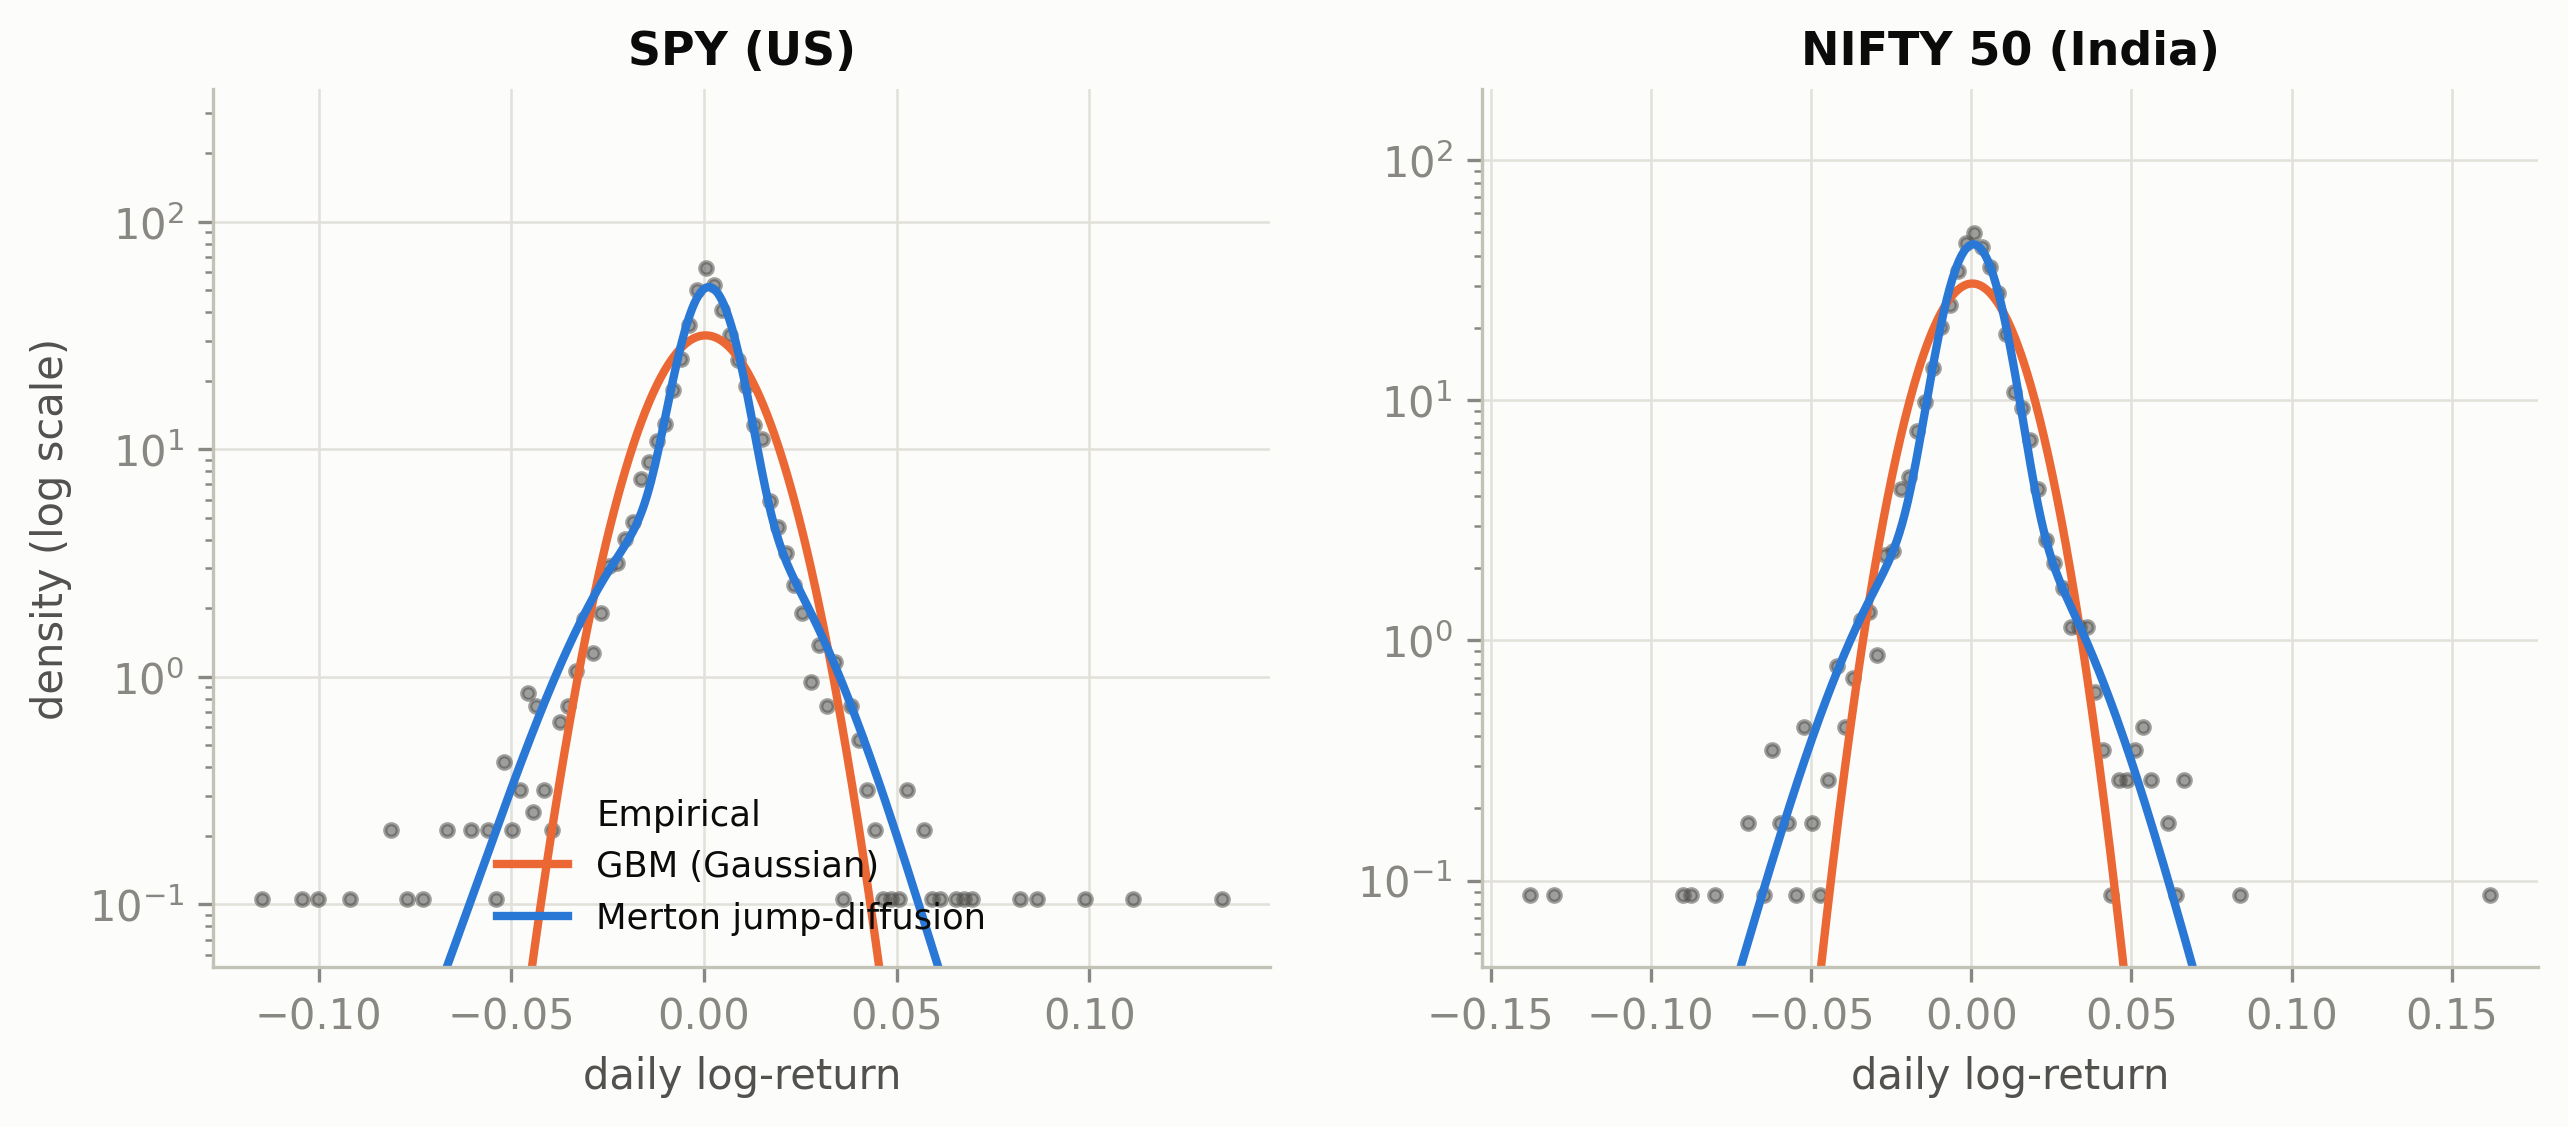
\includegraphics[width=\textwidth]{figs/fig1_densities.png}
\caption{Daily-return densities on a log scale: empirical (grey points), fitted GBM
(orange), fitted Merton (blue). The Gaussian collapses many decades too fast; the
jump mixture tracks the empirical tails on both markets.}
\label{fig:dens}
\end{figure}

\begin{figure}[h]\centering
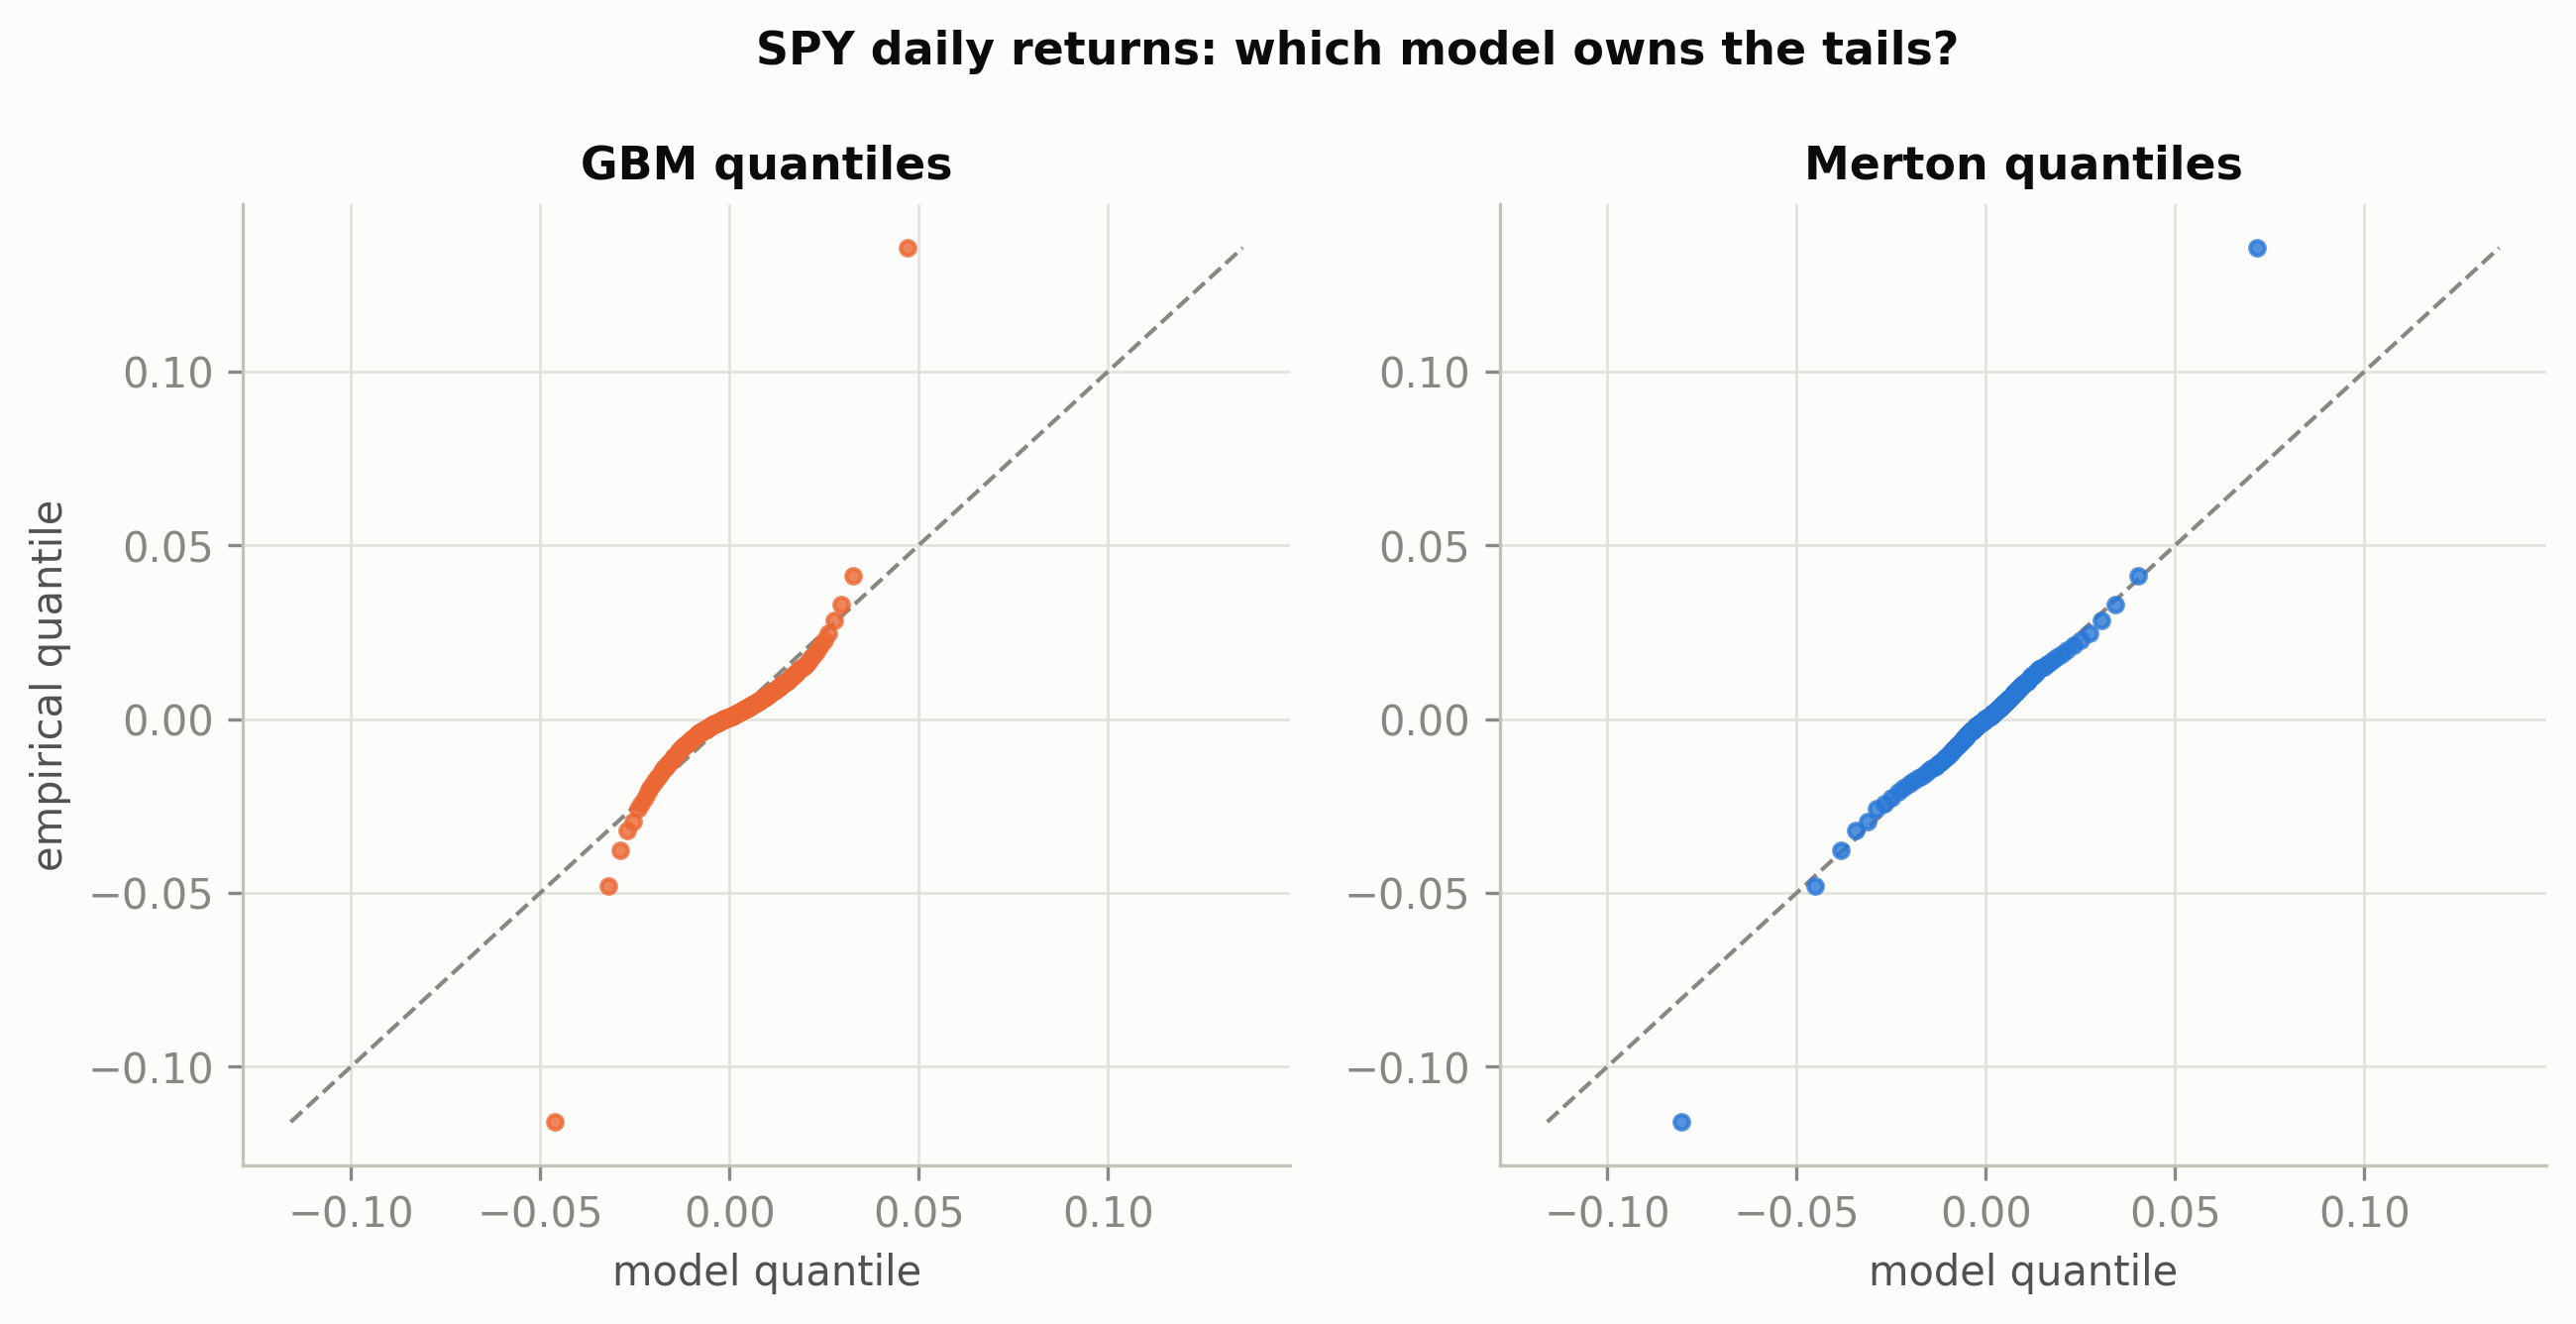
\includegraphics[width=\textwidth]{figs/fig2_qq_spy.png}
\caption{QQ plots of SPY daily returns against each fitted model. Against GBM the
empirical quantiles peel violently off the diagonal in both tails; against Merton
they hug it.}
\label{fig:qq}
\end{figure}

%=====================================================================
\section{Calibration II: the risk-neutral measure}
\label{sec:rn}

Option prices reveal the \emph{market's} model. Quoting each option as its
Black--Scholes \textbf{implied volatility} (the $\sigma$ that reproduces its price),
a Gaussian world would produce a flat line across strikes; real markets produce a
\textbf{skew} --- out-of-the-money puts trade at much higher implied vols, because
the market pays up for crash insurance.

For each snapshot we take the expiry nearest 90 days, keep OTM quotes with positive
bids (the liquid side of the smile), compute mid-price implied vols by Brent
root-finding (quotes violating no-arbitrage bounds are dropped), and fit Merton
parameters by weighted least squares on the smile:
\begin{equation}
\min_{\sigma,\lambda,\mu_J,\sigma_J}\;\sum_i w_i\,
\big(IV_M(K_i)-IV_{\text{mkt}}(K_i)\big)^2,\qquad
w_i\propto \exp\!\Big[-\tfrac12\big(\tfrac{\ln(K_i/S)}{0.15}\big)^2\Big],
\label{eq:rnobj}
\end{equation}
ATM-centred weights because at-the-money quotes carry the most information per unit
of noise (highest vega). For speed the optimiser uses the standard first-order
equivalence $\Delta IV \approx \Delta\text{price}/\text{vega}$ with vega frozen at
market IVs; the reported fit quality is recomputed by exact inversion.

\begin{table}[h]
\centering\small
\caption{Risk-neutral Merton calibrated to four real SPY chains ($\approx$90 DTE,
OTM quotes).}
\label{tab:rn}
\begin{tabular}{lccccccc}
\toprule
Snapshot & Regime & ATM IV & $\sigma$ & $\lambda$/yr & $\mu_J$ & $\sigma_J$ &
RMSE (vol pts)\\
\midrule
2017-01-03 & calm bull & 13.5\% & 0.068 & 0.92 & $-0.106$ & 0.100 & 1.27\\
2020-03-16 & COVID crash & 64.2\% & 0.116 & 3.68 & $-0.308$ & 0.190 & 0.74\\
2022-06-13 & bear market & 30.1\% & 0.128 & 2.00 & $-0.162$ & 0.136 & 0.67\\
2025-06-30 & recent & 14.3\% & 0.080 & 0.81 & $-0.138$ & 0.115 & 1.05\\
\bottomrule
\end{tabular}
\end{table}

\textbf{Reading Table~\ref{tab:rn}.} Even the calmest market prices roughly one
$-10\%$ jump per year --- the smile \emph{never} believes Black--Scholes. In March
2020 the market priced $\lambda=3.7$ crashes/year of mean $-31\%$. A 4-parameter
model reproduces 40+ vol-point skews to within about one vol point
(Figure~\ref{fig:smiles}). These COVID-chain parameters --- a jump world someone
actually paid for --- define the ``true world'' of the mismatch experiments.

\begin{figure}[h]\centering
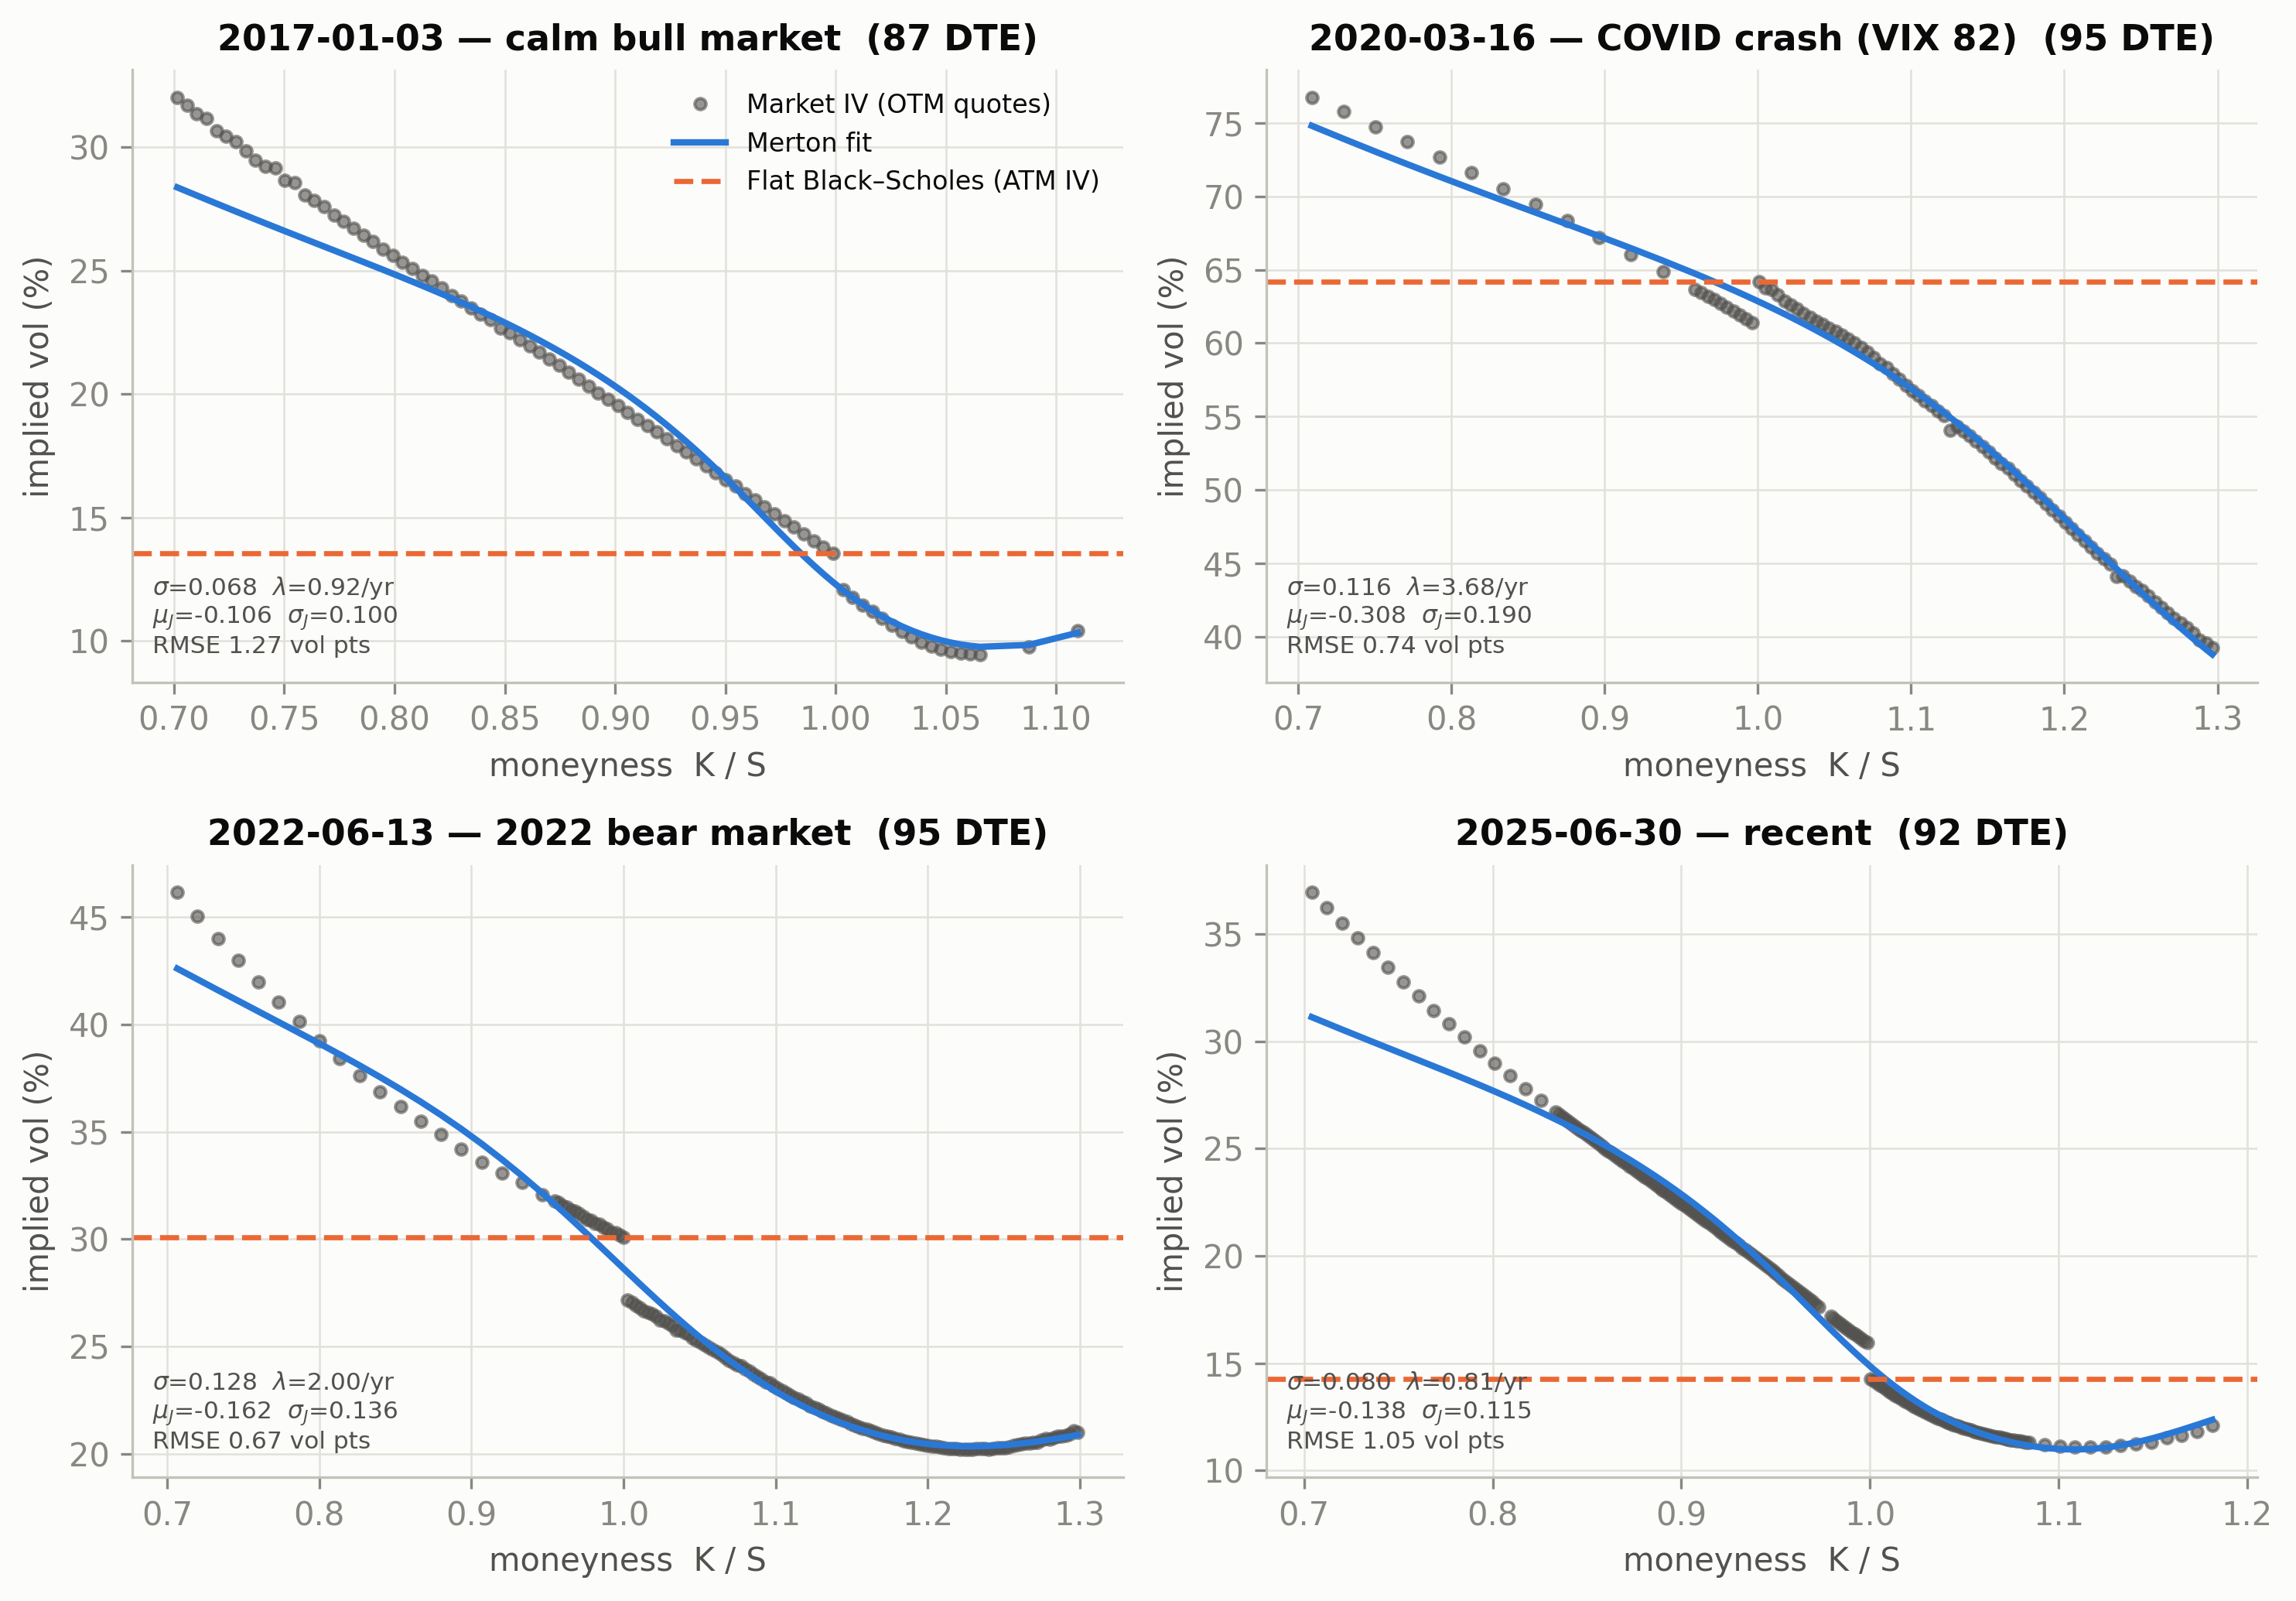
\includegraphics[width=\textwidth]{figs/fig3_smiles.png}
\caption{Real SPY implied-vol skews (grey), Merton fits (blue), and the flat smile
Black--Scholes implies (orange dashed), on four dates spanning calm to crisis.}
\label{fig:smiles}
\end{figure}

%=====================================================================
\section{The desk: generating market-making P/L under model risk}
\label{sec:desk}

\subsection{Mechanics}
Time advances in ticks ($dt=1/250$ years). At each tick the desk quotes a
\emph{fresh} option with constant maturity $T=3$ months and strike at current spot
($K_t=S_t$): rolling constant moneyness keeps the business stationary --- a fixed
strike would drift out of the money as the underlying trends, silently shrinking
both risk and revenue and contaminating every downstream statistic (this exact
artefact was caught by a failing coverage backtest during development and is
documented in the repo history). Around its believed fair value it posts
$\text{bid}=V_{\text{mod}}-s$, $\text{ask}=V_{\text{mod}}+s$.

When a client trades, the contract's P/L is \textbf{realised at the fill}: the
underlying is simulated over the option's life under the \emph{true} model
(GBM or Merton), while the desk delta-hedges at 30 rebalance dates using \emph{its
own} model's delta, financing the hedge at $r$; premium, hedge cash flows and
terminal payoff are discounted to the fill date. Realising at the fill keeps the
equity curve a story about \emph{pricing edge}, not about an ever-growing open
inventory position.

\subsection{Why a hedged option earns ``premium minus fair value''}
For a delta-hedged short option rebalanced continuously under the model's own
dynamics, the $\dd W$ terms cancel and the hedged portfolio grows at $r$; the
discounted P/L of (sell at premium $p$, hedge to expiry) converges to
\begin{equation}
\text{P/L}\;\longrightarrow\;p-V_{\text{fair}},
\label{eq:hedgedpnl}
\end{equation}
\emph{independent of the drift} $\mu$. Selling at $V+s$ or buying at $V-s$ then
banks $+s$ per contract in expectation. Model error breaks both legs of this
argument simultaneously: the quotes centre on the wrong $V$ (a systematic,
sign-definite error), and the hedge follows the wrong delta --- worse, \emph{no}
delta hedge can follow a jump, because the price gaps a finite amount in an
instant. Two further honest caveats: with 30 discrete rebalances the cancellation
in \eqref{eq:hedgedpnl} is approximate (mean-zero noise remains), and under jumps
the market is \emph{incomplete} --- even the right-model desk retains
undiversifiable jump risk plus a small residual drift exposure, which is why its
realised edge in Table~\ref{tab:desk} ($0.194$) sits slightly above the quoted
$0.15$ rather than exactly on it.

\subsection{Elastic client flow: mispricing attracts sharks}
Real clients compare quotes to value. Each side's fill probability is scaled by how
bad the quote is for the client, in units of half-spread against \emph{true} fair
value:
\begin{equation}
p_{\text{fill}}=\min\!\Big(0.98,\;p_0\,
e^{-\eta\cdot\text{excess}}\Big),\qquad
\text{excess}_{\text{ask}}=\frac{\text{ask}-V_{\text{true}}}{s}-1,
\label{eq:elastic}
\end{equation}
capped at $e^{2}\times$ the base rate (client arrival is finite even when the desk
gives money away). A fairly-priced quote trades at the base rate; a rich quote
loses business; a cheap quote is run over by informed flow --- adverse selection.
Flow is put-heavy (base $\Prob(\text{client buys})=0.5$ vs $\Prob(\text{client
sells})=0.1$ per tick), matching the real net demand for index crash protection,
so a desk that underprices puts ends up systematically \emph{short} crash
insurance. Without elasticity ($\eta=0$) the simulator reproduces the textbook
version where an overpricing desk looks brilliant; with it, both directions of
mispricing are punished --- which is what Table~\ref{tab:desk} shows.

\subsection{The four scenarios}
All use $S_0=100$, ATM puts, $T=0.25$, $r=2\%$, $\mu=6\%$, $s=0.15$, 250 ticks
(one year), seeds $0..n-1$:
\begin{itemize}[itemsep=1pt]
\item \textbf{Matched}: world GBM ($\sigma=0.20$, the SPY fit); desk prices
  Black--Scholes with the same $\sigma$.
\item \textbf{Steamroller}: world Merton with the COVID-chain parameters
  ($\sigma=0.116,\lambda=3.68,\mu_J=-0.308,\sigma_J=0.19$); desk prices
  Black--Scholes with only the diffusive $\sigma$.
\item \textbf{Right model}: world as above; desk prices Merton with the true
  parameters.
\item \textbf{Overcautious}: world GBM; desk prices Merton with COVID jumps that
  never come.
\end{itemize}

%=====================================================================
\section{Results I: P/L distributions and the price of model risk}
\label{sec:risk}

\begin{table}[h]
\centering\small
\caption{Desk experiments across seeds. Edge CI is a 95\% percentile bootstrap on
per-seed average realised edge per contract. Negative VaR/ES means the 5\% tail is
still a profit.}
\label{tab:desk}
\begin{tabular}{lcccccc}
\toprule
Scenario & Seeds & Believed edge & Realised edge [95\% CI] & Mean P/L &
VaR$_{5\%}$ & ES$_{5\%}$\\
\midrule
Matched & 300 & $+0.15$ & $+0.153\;[0.146, 0.159]$ & $+22.8$ & $-9.4$ & $-4.0$\\
Right model & 200 & $+0.15$ & $+0.194\;[0.064, 0.324]$ & $+28.3$ & $207.9$ & $289.7$\\
Steamroller & 300 & $+0.15$ & $-10.20\;[-10.62, -9.78]$ & $-2497.8$ & $4012.5$ & $4466.9$\\
Overcautious & 200 & $+0.15$ & $-9.08\;[-9.23, -8.92]$ & $-1671.1$ & $2044.7$ & $2127.9$\\
\bottomrule
\end{tabular}
\end{table}

\textbf{Reading Table~\ref{tab:desk}.} Three lessons. (i)~The matched desk delivers
exactly what it promises --- realised edge statistically indistinguishable from the
quoted half-spread. (ii)~The mismatched desks lose catastrophically \emph{in both
directions}: underpricing is picked off by buyers of cheap crash insurance
(steamroller), overpricing is picked off by sellers dumping overpriced options on
the desk's rich bid (overcautious). Model risk is not ``being too cheap''; it is
\emph{being wrong in either direction when the other side knows better}. (iii)~Even
the right-model desk in a jump world carries much fatter P/L tails than the matched
desk (incomplete market: jumps cannot be hedged away), which is a fact about
markets, not a bug.

\begin{figure}[h]\centering
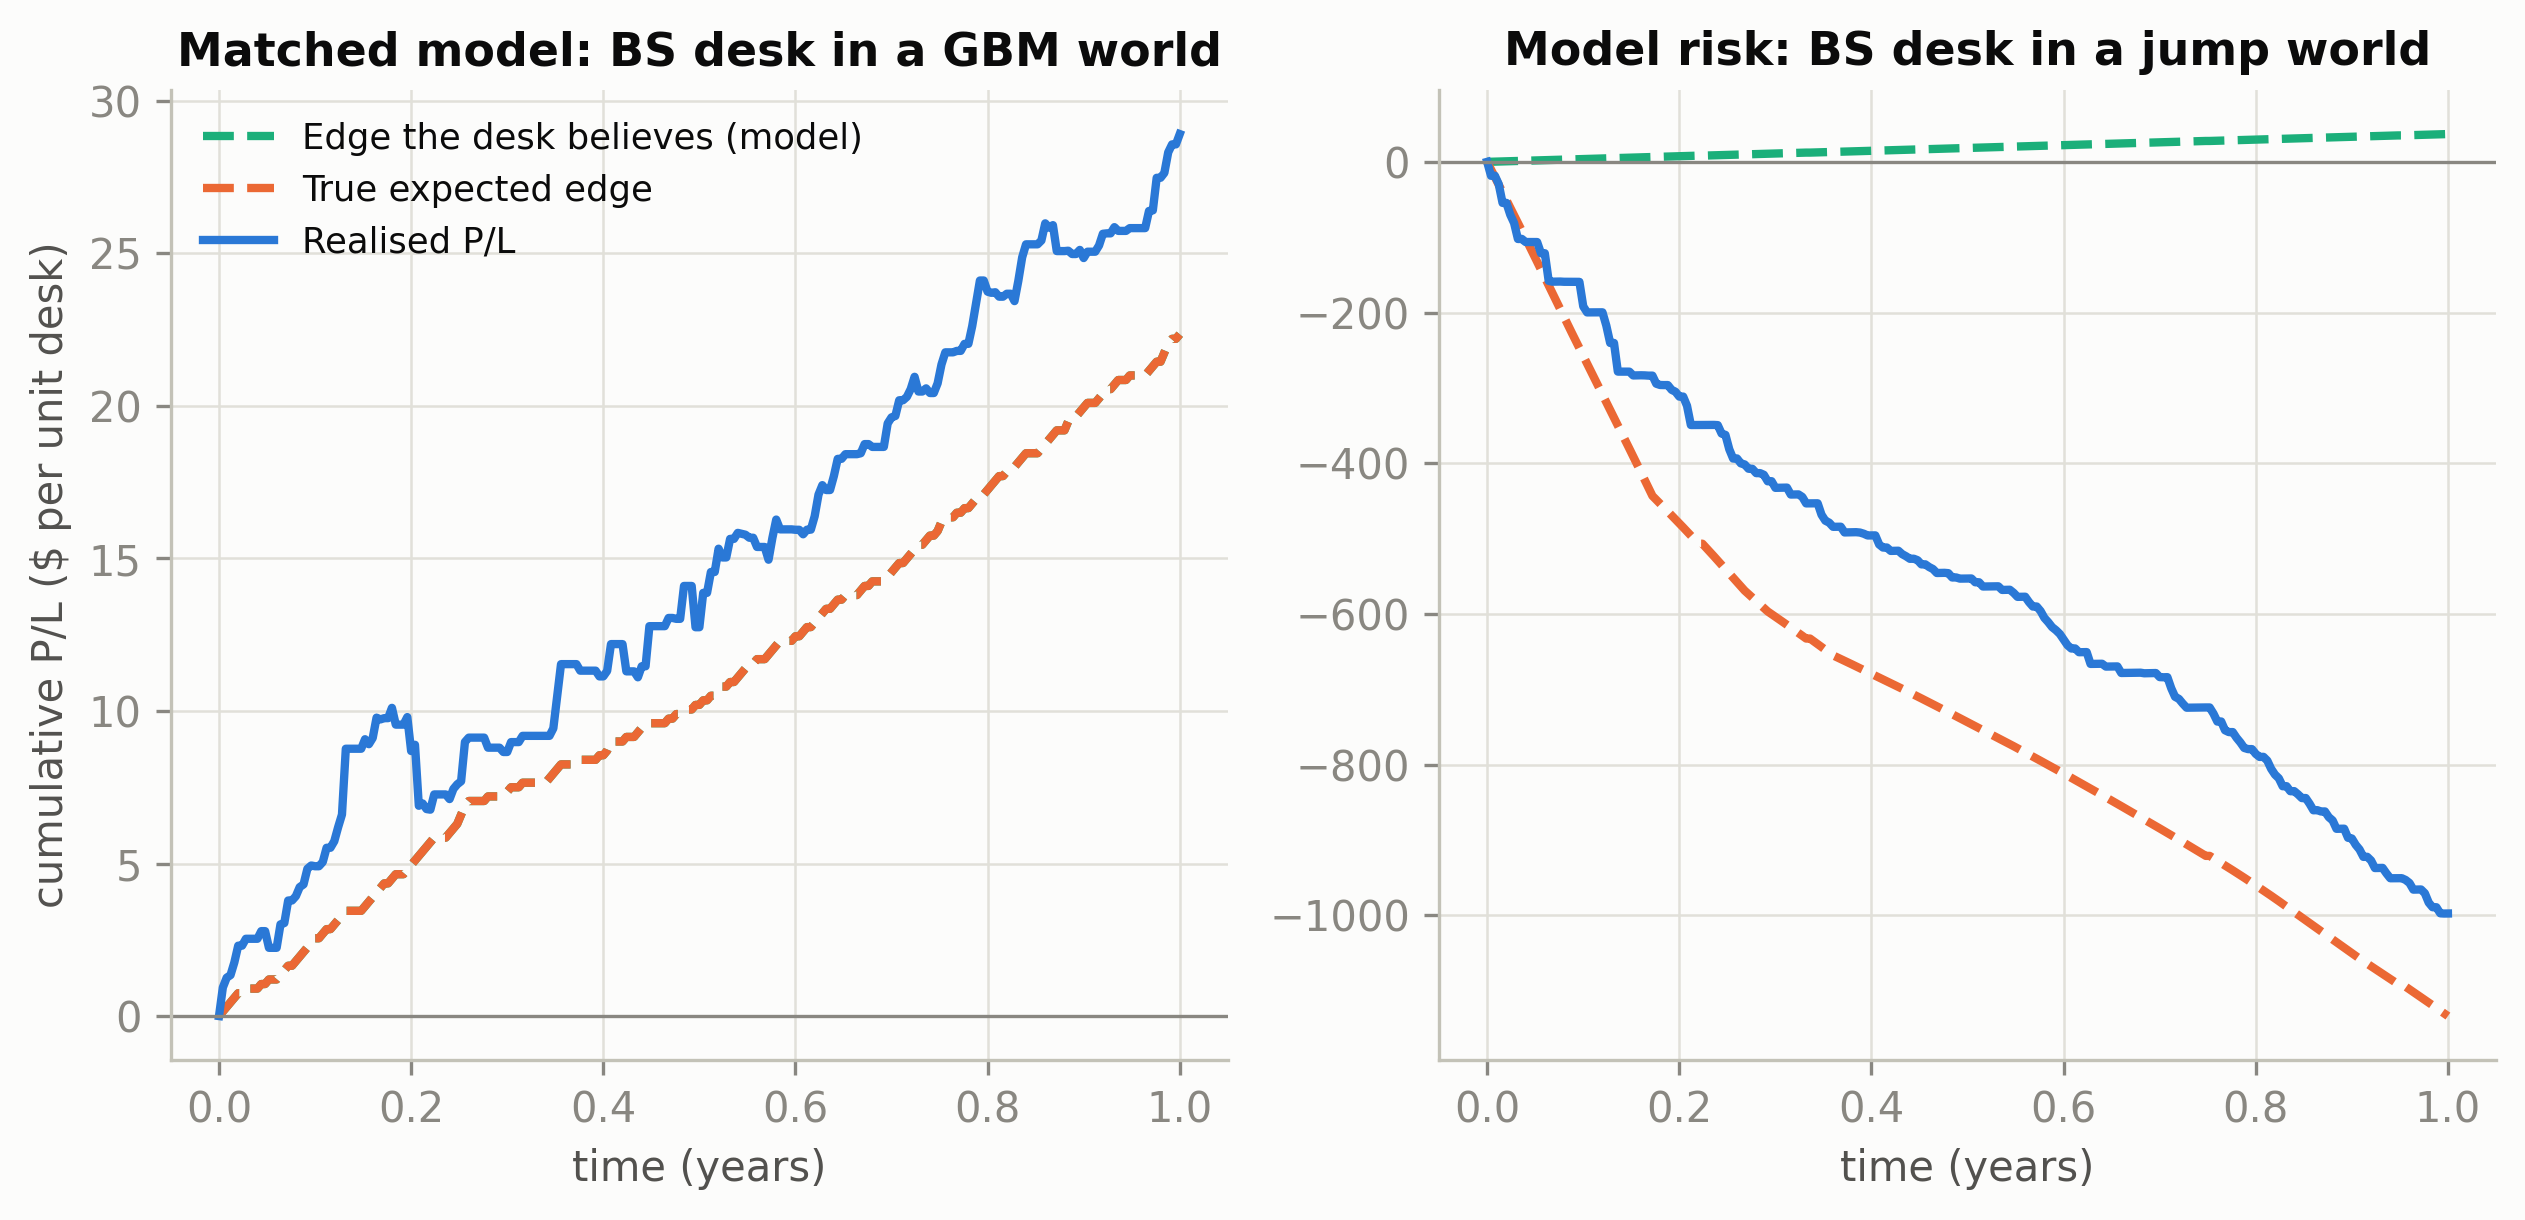
\includegraphics[width=\textwidth]{figs/fig4_equity.png}
\caption{One seed, two worlds. Left: matched desk --- realised P/L rides the
believed and true edge lines. Right: steamroller --- the desk's own accounting
(teal, top) reports steady profit while true expectation and realised P/L collapse.
The vertical gap \emph{is} model risk in dollars.}
\label{fig:equity}
\end{figure}

\begin{figure}[h]\centering
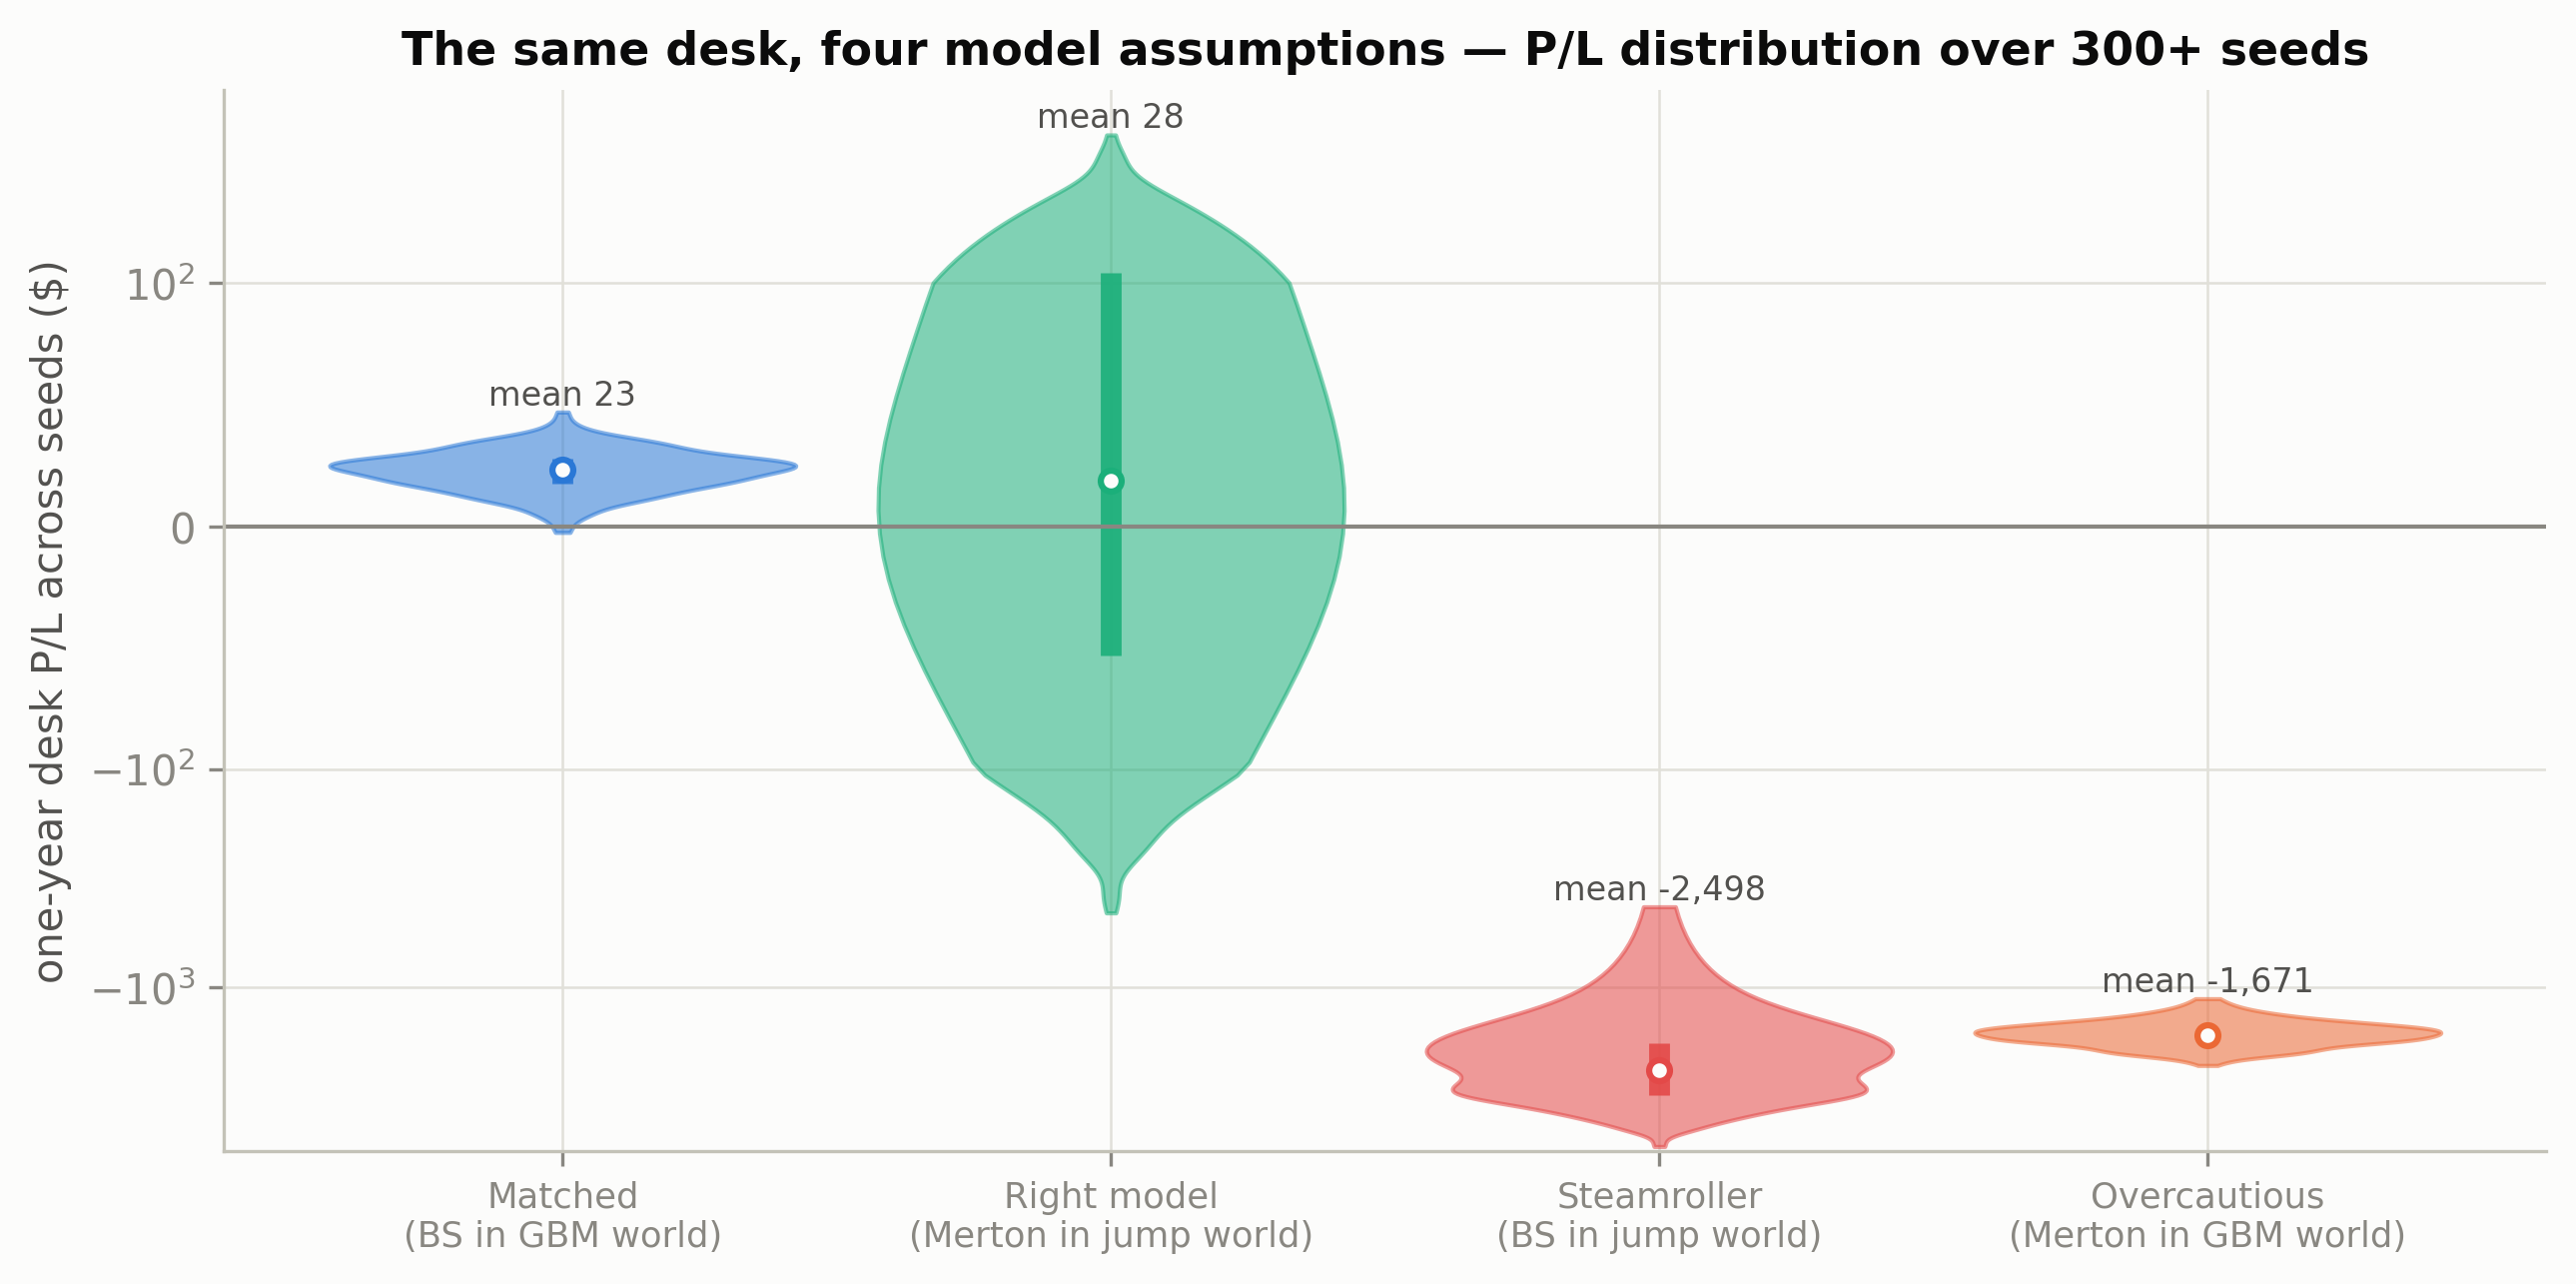
\includegraphics[width=\textwidth]{figs/fig5_pnl_distributions.png}
\caption{One-year P/L across seeds, all four scenarios (symlog scale).}
\label{fig:dists}
\end{figure}

\subsection{The model-risk premium}
Re-running the desk over a grid of half-spreads traces the loss-probability curve
$s\mapsto\Prob(\text{P/L}(s)<0)$ (Figure~\ref{fig:breakeven}). Define the
break-even spread as the smallest $s$ with $\Prob(\text{loss})\le5\%$:
\begin{keybox}
\textbf{Matched desk: breaks even at $s^\ast=8.8$ cents.}\\
\textbf{Mispriced desk: no break-even below \$15} --- more than $170\times$ wider.
With informed (elastic) flow, widening the quote throttles the business faster
than it buys safety: the desk cannot spread its way out of a wrong model.
\end{keybox}
This is the project's answer to ``what does model risk cost'': for this desk, the
model-risk premium is not a few extra cents of spread --- it is the difference
between a viable business and no business at all.

\begin{figure}[h]\centering
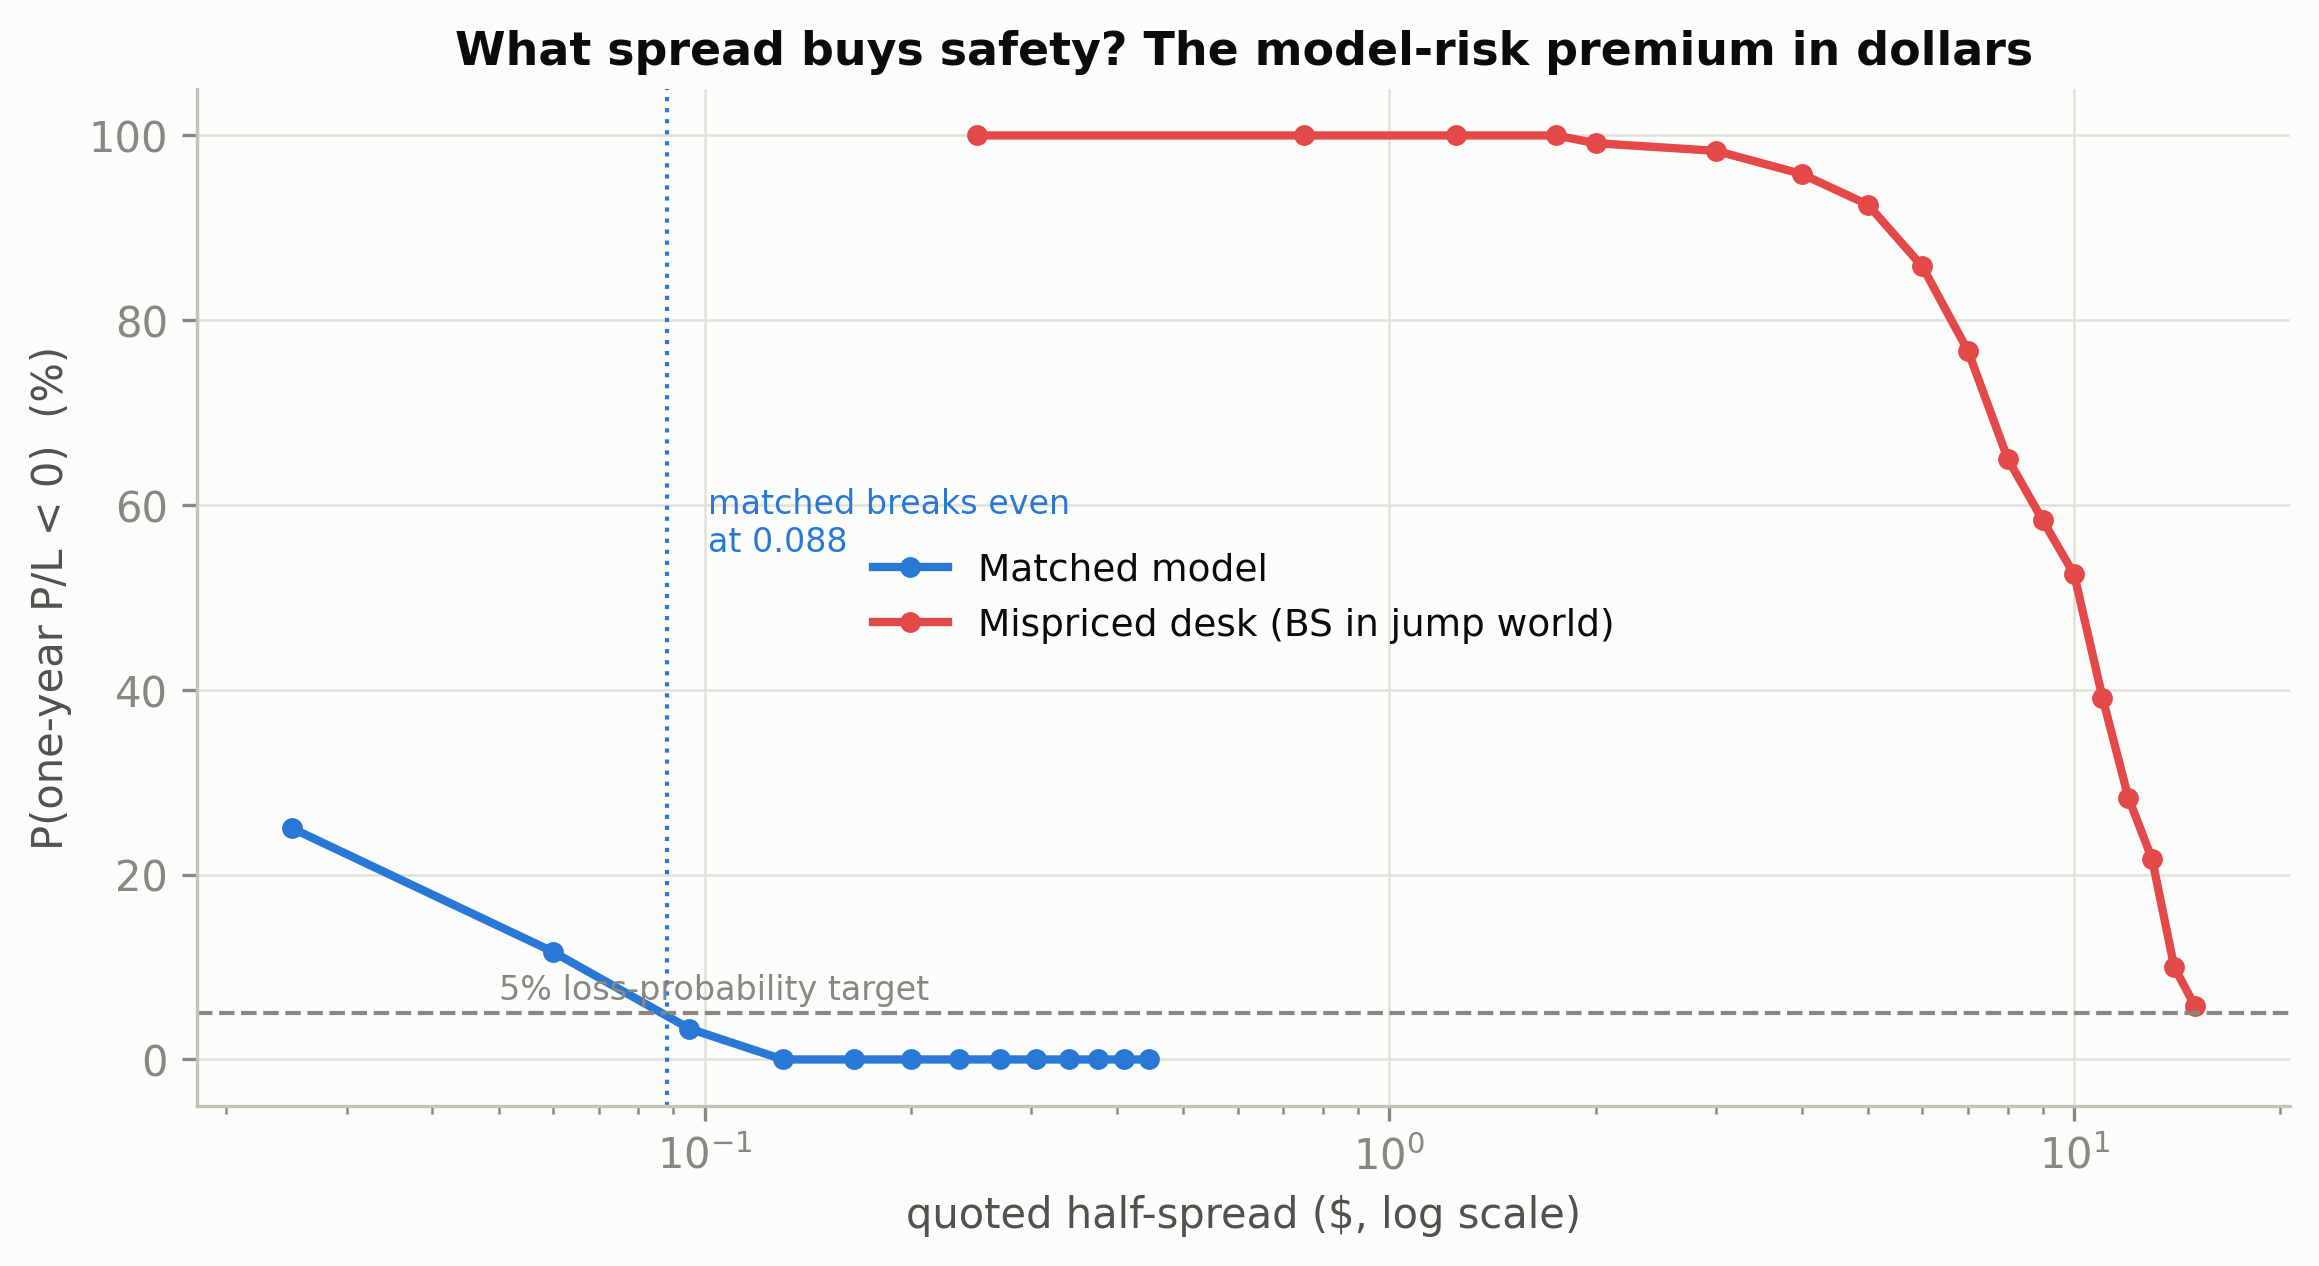
\includegraphics[width=0.85\textwidth]{figs/fig6_breakeven.png}
\caption{Loss probability vs quoted half-spread (log scale).}
\label{fig:breakeven}
\end{figure}

%=====================================================================
\section{Results II: validation --- catching the wrong model from P/L alone}
\label{sec:validation}

A model validator does not get to observe ``the true model''; they observe
\emph{outcomes}. This section runs the standard MRM toolkit on the desk's realised
P/L, on a six-year run (1{,}500 ticks) for test power. To keep the P/L series
stationary, all per-tick quantities are scaled by the spot level (risk per unit of
notional --- an ATM option's dollar value is proportional to $S$).

\subsection{Kupiec's proportion-of-failures (POF) test}
The desk forecasts its own 5\% one-tick VaR by simulating its \emph{believed} world
(the standard model-based VaR practice). If the model is right, losses should
exceed VaR on $\alpha=5\%$ of ticks, independently. Observing $x$ exceptions in $n$
ticks:
\begin{equation}
LR_{\text{pof}}
=-2\ln\frac{(1-\alpha)^{n-x}\alpha^{x}}{(1-\hat\pi)^{n-x}\hat\pi^{x}}
\;\overset{H_0}{\sim}\;\chi^2_1,\qquad \hat\pi=x/n .
\end{equation}

\subsection{Christoffersen's independence and conditional coverage}
Correct frequency is not enough --- exceptions must not \emph{cluster}. Model the
exception indicator as a two-state Markov chain with transition counts $n_{ij}$
and conditional exception probabilities $\pi_0,\pi_1$; test $\pi_0=\pi_1$:
\begin{equation}
LR_{\text{ind}}=-2\ln\frac{(1-\hat\pi)^{n_{00}+n_{10}}\hat\pi^{\,n_{01}+n_{11}}}
{(1-\hat\pi_0)^{n_{00}}\hat\pi_0^{\,n_{01}}(1-\hat\pi_1)^{n_{10}}\hat\pi_1^{\,n_{11}}}
\overset{H_0}{\sim}\chi^2_1,
\qquad LR_{cc}=LR_{\text{pof}}+LR_{\text{ind}}\overset{H_0}{\sim}\chi^2_2 .
\end{equation}
Clustered exceptions are the signature of dynamics the model does not have ---
here, jumps.

\subsection{Bootstrap inference on realised edge}
Per-seed average edges are i.i.d.\ by construction, so a percentile bootstrap
(10{,}000 resamples) gives honest confidence intervals for mean edge, reported in
Table~\ref{tab:desk}, alongside a one-sample $t$-test of $H_0$: mean edge $=0$.

\subsection{CUSUM: the early-warning monitor}
Waiting a year for a backtest is a luxury; a desk bleeding edge should be caught in
weeks. The one-sided CUSUM tracks cumulative under-delivery of the promised edge
$m$ on spot-scaled per-trade residuals $X_t$:
\begin{equation}
C_0=0,\qquad C_t=\max\big(0,\;C_{t-1}+(m-X_t)-k\big),
\qquad\text{alarm when } C_t>h,
\end{equation}
with allowance $k=0.5\hat\sigma$ and threshold $h=8\hat\sigma$, control limits
calibrated on a burn-in window that is excluded from monitoring (you do not raise
alarms on the data used to set the limits).

\begin{table}[h]
\centering\small
\caption{Validation results on six-year runs (1{,}500 ticks; expected exceptions
75).}
\label{tab:validation}
\begin{tabular}{lccc}
\toprule
Test & Matched desk & Mispriced desk & Verdict\\
\midrule
Kupiec POF & 83 exc., $p=0.351$ & 811 exc., $p<10^{-16}$ &
right model passes; wrong fails\\
Christoffersen CC & $p=0.619$ & $p<10^{-16}$ & wrong model's exceptions cluster\\
CUSUM & no alarm in 903 trades & alarm at trade \textbf{83} of 1{,}467 &
detection in $\sim$3 weeks\\
\bottomrule
\end{tabular}
\end{table}

\begin{figure}[h]\centering
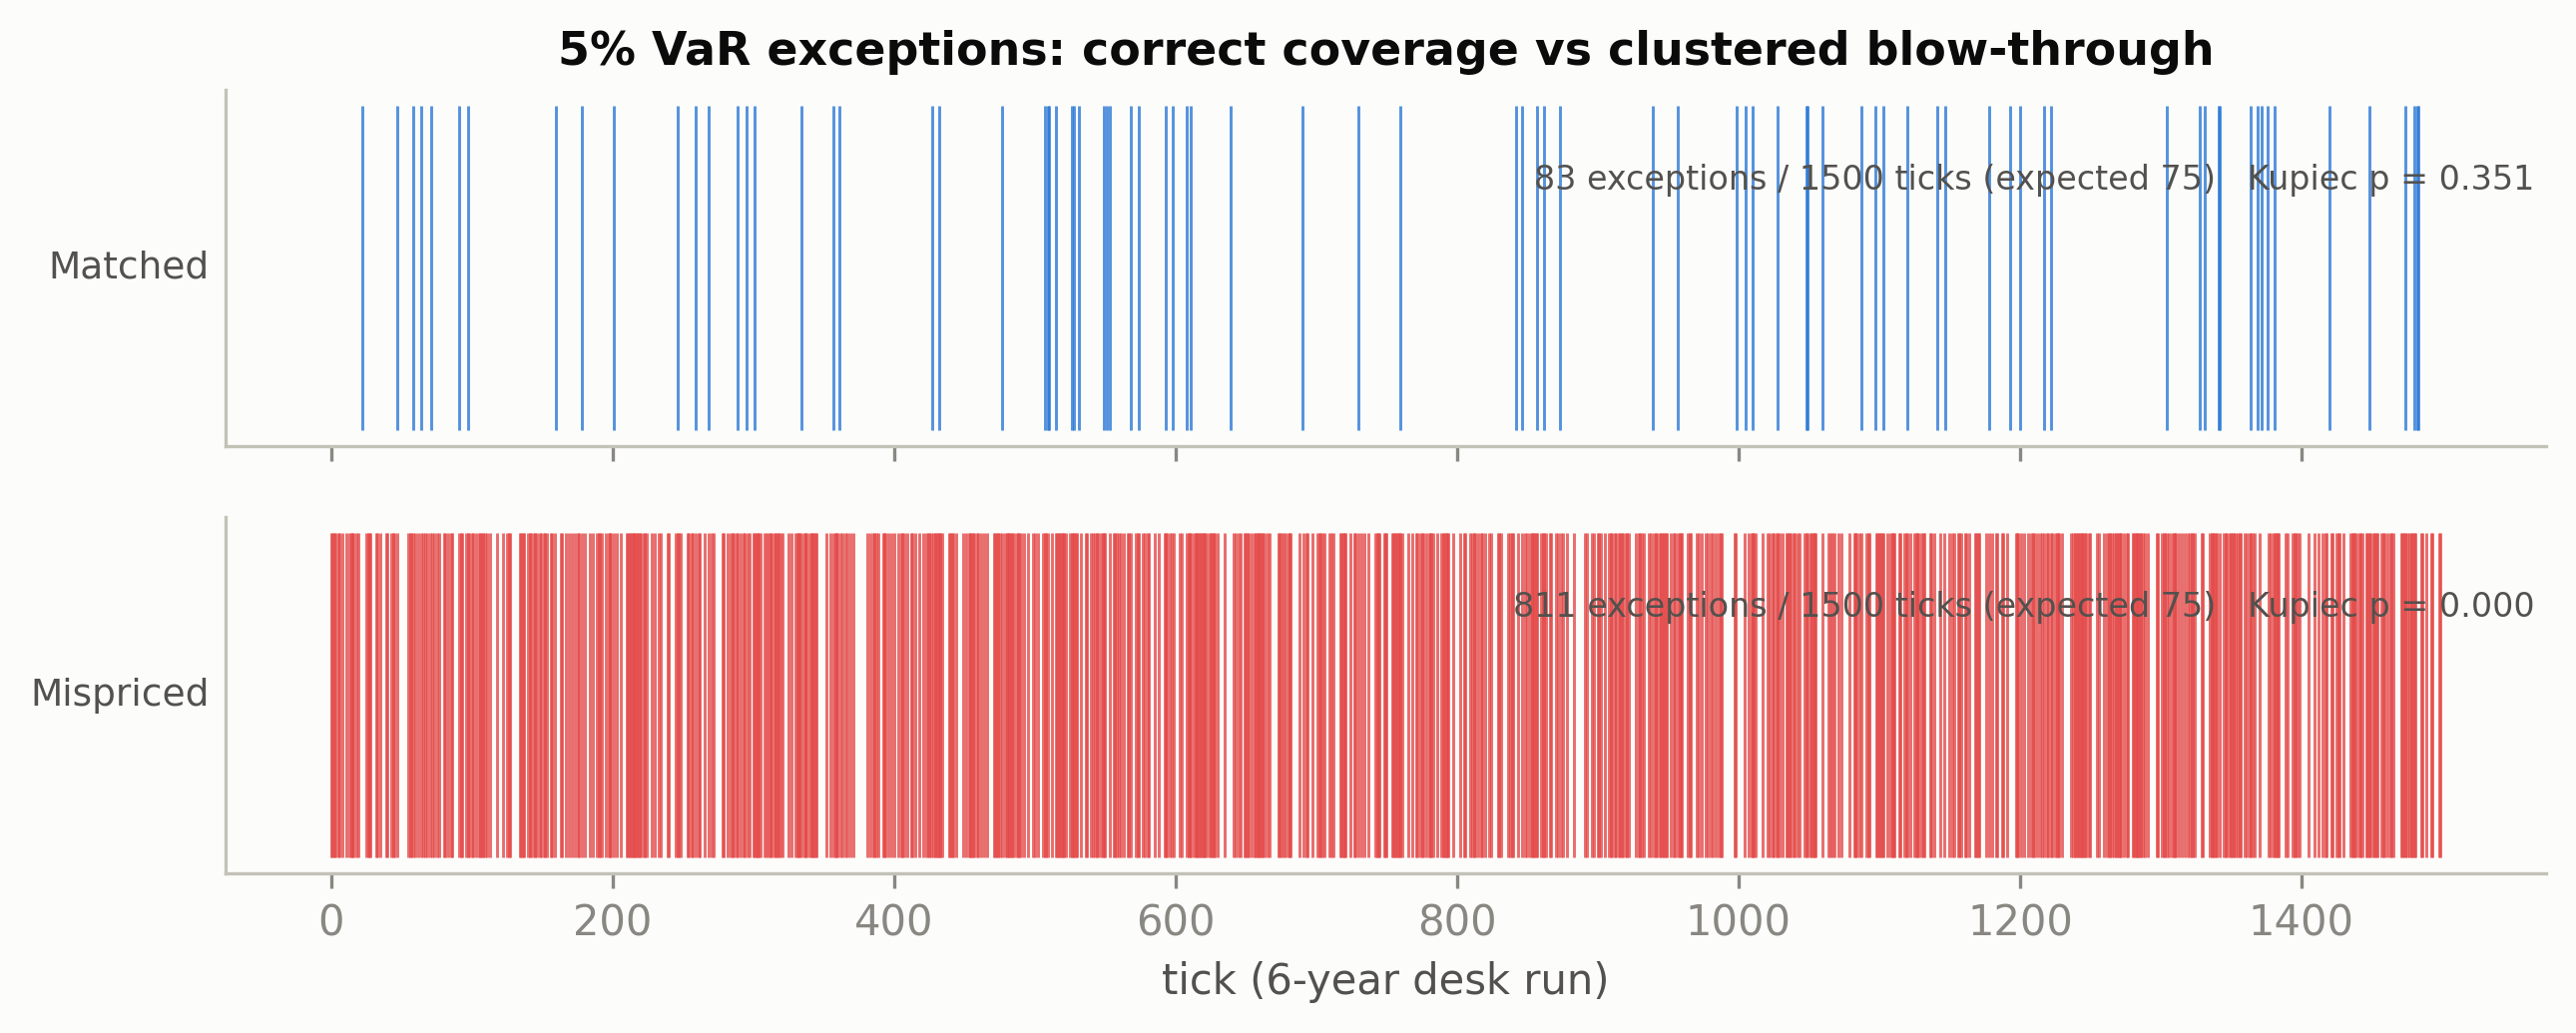
\includegraphics[width=\textwidth]{figs/fig8_var_exceptions.png}
\caption{5\% VaR exception timelines. Matched: 83 scattered exceptions vs 75
expected. Mispriced: 811, clustered into jump episodes.}
\label{fig:exceptions}
\end{figure}

\begin{figure}[h]\centering
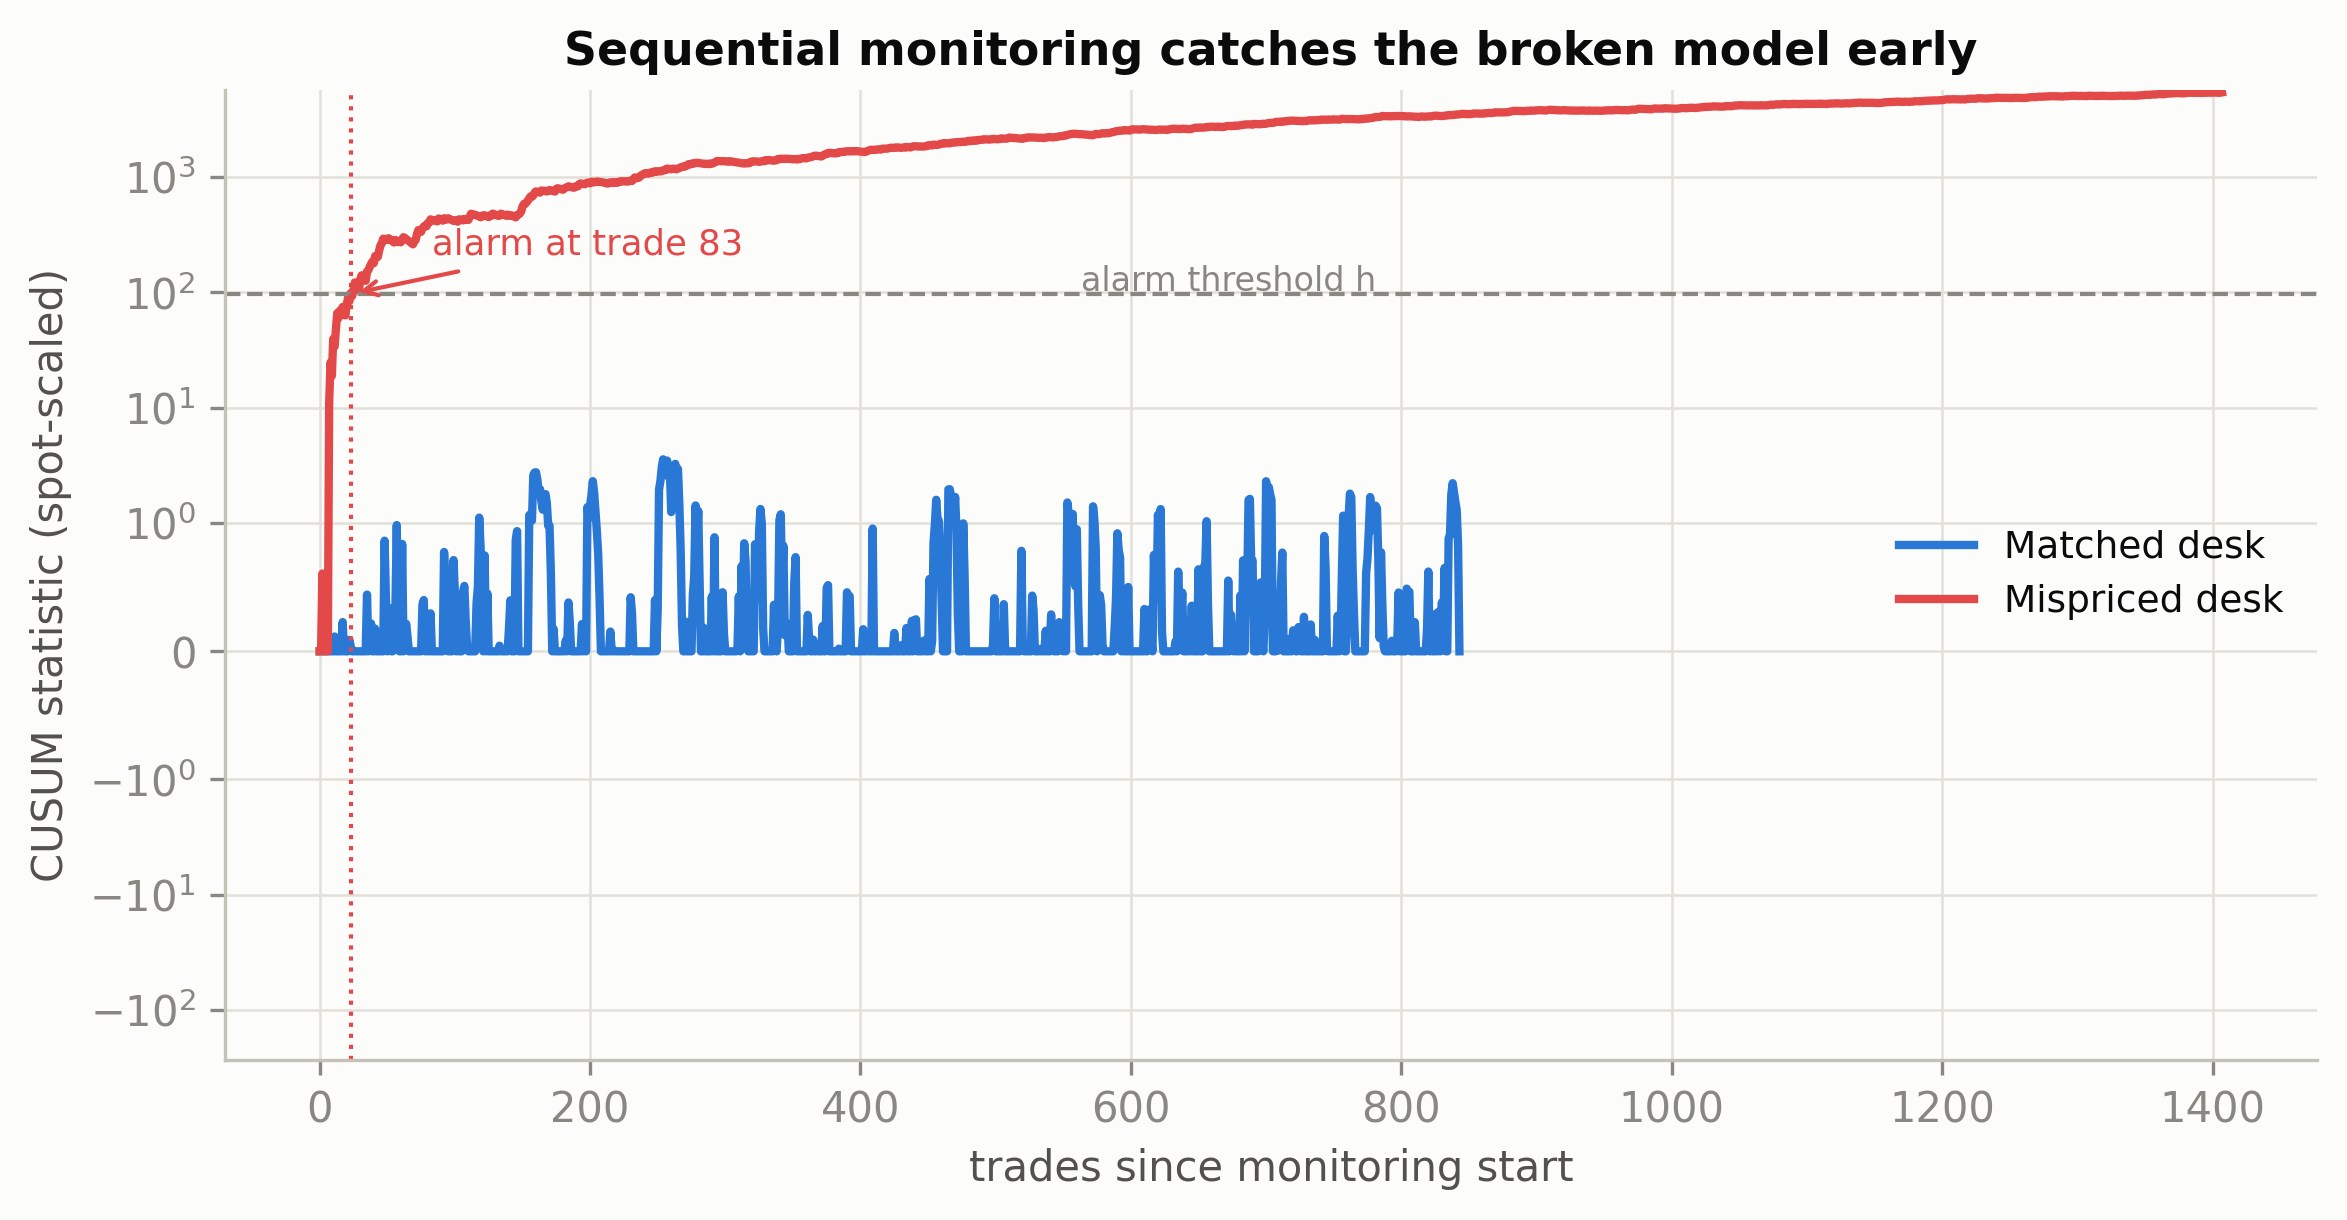
\includegraphics[width=0.9\textwidth]{figs/fig7_cusum.png}
\caption{CUSUM paths. The matched desk's statistic breathes below threshold for
900+ trades (zero false alarms); the mispriced desk crosses at trade 83.}
\label{fig:cusum}
\end{figure}

\begin{keybox}
\textbf{The validator's takeaway.} The wrong model is not merely unprofitable ---
it is \emph{statistically detectable} from realised P/L, quickly, with tests whose
false-alarm behaviour is verified on the correctly-specified desk. This is the
entire logic of model risk management, demonstrated end to end on one desk.
\end{keybox}

%=====================================================================
\section{Limitations, stated plainly}
\label{sec:limitations}
\begin{itemize}[itemsep=2pt]
\item \textbf{Stylised microstructure.} One contract, Bernoulli client arrivals, a
  reduced-form elasticity \eqref{eq:elastic} rather than an order book or a
  utility-based client model.
\item \textbf{Static parameters within runs.} No stochastic volatility, no
  parameter drift; the ``truth'' inside each experiment is a fixed Merton world.
  Real model risk includes the model being wrong \emph{in form}, not only in
  parameters --- our mismatch captures exactly one axis of that.
\item \textbf{Boundary null in the LR test} (Section~\ref{sec:physical});
  conclusions are robust here but the caveat matters at smaller samples.
\item \textbf{Incomplete-market subtleties} under jumps: hedged P/L is not fully
  drift-free, and jump risk premia (difference between $P$- and $Q$-measure jump
  parameters) are real economics that the right-model desk partially collects; a
  full treatment would separate them explicitly.
\item \textbf{Data vintage.} Chains end December 2025; NIFTY options are not in
  the free mirror used (the repo ships a fetch script for NSE data to extend the
  Indian leg).
\end{itemize}
None of these change the qualitative conclusions; each is a natural extension.

%=====================================================================
\section{Reproducibility}
\label{sec:repro}
Everything regenerates from two commands:
\begin{center}
\texttt{python scripts/run\_experiments.py} \quad$\rightarrow$\quad
\texttt{python scripts/make\_figures.py}
\end{center}
Deterministic seeds throughout; 15 unit tests (put--call parity, delta vs finite
differences, Merton $\to$ BS convergence, MLE recovery on synthetic data, matched
desk realising its half-spread, Kupiec/Christoffersen/CUSUM behaviour on synthetic
series) run via \texttt{python -m pytest tests/}. The interactive website ports the
same engine to JavaScript with a seeded RNG. Repository:
\url{https://github.com/Arijitray2/model-risk-lab}.

%=====================================================================
\section*{References}
\begin{itemize}[itemsep=1pt,label={}]
\item Black, F., Scholes, M. (1973). The Pricing of Options and Corporate
  Liabilities. \emph{JPE} 81(3).
\item Merton, R.C. (1976). Option pricing when underlying stock returns are
  discontinuous. \emph{JFE} 3(1--2).
\item Kupiec, P. (1995). Techniques for Verifying the Accuracy of Risk Measurement
  Models. \emph{J. Derivatives} 3(2).
\item Christoffersen, P. (1998). Evaluating Interval Forecasts. \emph{IER} 39(4).
\item Page, E.S. (1954). Continuous Inspection Schemes. \emph{Biometrika} 41.
\item Board of Governors of the Federal Reserve (2011). SR 11-7: Guidance on Model
  Risk Management.
\item Paolucci, R. --- Quant Guild (2026). \emph{Projects to Help you Become a
  Quant (Intermediate)} --- the teaching simulator this project modifies and
  extends.
\end{itemize}

\end{document}
